%%%% ijcai20.tex

\typeout{IJCAI--PRICAI--20 Instructions for Authors}

% These are the instructions for authors for IJCAI-20.

\documentclass{article}
\pdfpagewidth=8.5in
\pdfpageheight=11in
% The file ijcai20.sty is NOT the same than previous years'
\usepackage{ijcai20}

% Use the postscript times font!
\usepackage{times}
\usepackage{latexsym}
\usepackage{soul}
\usepackage{url}
\usepackage[draft]{hyperref}
%\usepackage[small]{caption}
\usepackage{graphicx}
\usepackage{amsmath}
\usepackage{amsthm}
\usepackage{booktabs}
\usepackage{algorithm}
\usepackage{algorithmic}
\usepackage{helvet}
\usepackage{courier}
\usepackage{color}
\usepackage{amsmath,amsfonts,amssymb,amsthm,amsopn}
\usepackage{epsfig}
\usepackage{graphicx}
\usepackage{booktabs}
\usepackage{array}
\usepackage{multicol}
\usepackage{threeparttable}
\usepackage{epstopdf}
\usepackage{listings}
\usepackage{multirow}
\usepackage{subfigure}
\usepackage{ragged2e}
\urlstyle{same}
\newcommand{\figref}[1]{Figure \ref{#1}}
\newcommand{\eqnref}[1]{Eq. \ref{#1}}
\newcommand{\tabref}[1]{Table \ref{#1}}
\newcommand{\secref}[1]{Section \ref{#1}}
\newcommand{\algoref}[1]{Algorithm \ref{#1}}
\renewcommand\appendix{\setcounter{secnumdepth}{3}}
\newcommand{\KZ}[1]{\textcolor{blue}{Kenny: #1}}
\newcommand{\SY}[1]{\textcolor{red}{Sophie: #1}}
\newcommand{\ZL}[1]{\textcolor{red}{Zilu: #1}}
\newcommand{\Bran}[1]{\textcolor{magenta}{Bran: #1}}

% the following package is optional:
%\usepackage{latexsym} 

% See https://www.overleaf.com/learn/latex/theorems_and_proofs
% for a nice explanation of how to define new theorems, but keep
% in mind that the amsthm package is already included in this
% template and that you must *not* alter the styling.
\newtheorem{example}{Example}
\newtheorem{theorem}{Theorem}

\renewcommand{\raggedright}{\leftskip=0pt \rightskip=0pt plus 0cm}

% Following comment is from ijcai97-submit.tex:
% The preparation of these files was supported by Schlumberger Palo Alto
% Research, AT\&T Bell Laboratories, and Morgan Kaufmann Publishers.
% Shirley Jowell, of Morgan Kaufmann Publishers, and Peter F.
% Patel-Schneider, of AT\&T Bell Laboratories collaborated on their
% preparation.

% These instructions can be modified and used in other conferences as long
% as credit to the authors and supporting agencies is retained, this notice
% is not changed, and further modification or reuse is not restricted.
% Neither Shirley Jowell nor Peter F. Patel-Schneider can be listed as
% contacts for providing assistance without their prior permission.

% To use for other conferences, change references to files and the
% conference appropriate and use other authors, contacts, publishers, and
% organizations.
% Also change the deadline and address for returning papers and the length and
% page charge instructions.
% Put where the files are available in the appropriate places.

\title{AspectFAQ: Generating Questions and Answers from Text and an Aspect}

% Single author syntax
%\author{
%    Christian Bessiere
%    \affiliations
%    CNRS, University of Montpellier, France
%    \emails
%    pcchair@ijcai20.org
%}

% Multiple author syntax (remove the single-author syntax above and the \iffalse ... \fi here)
% Check the ijcai20-multiauthor.tex file for detailed instructions
\iffalse
\author{
First Author$^1$
\and
Second Author$^2$\and
Third Author$^{2,3}$\And
Fourth Author$^4$
\affiliations
$^1$First Affiliation\\
$^2$Second Affiliation\\
$^3$Third Affiliation\\
$^4$Fourth Affiliation
\emails
\{first, second\}@example.com,
third@other.example.com,
fourth@example.com
}
\fi

\begin{document}

\maketitle

\begin{abstract}
Aspect-based question-answer pairs generation aims at generating the 
meaningful and interesting question-answer pairs from a document and 
a specific angle. 
This is a brand new problem and no existing methods or datasets are designed specifically for this problem. 
This problem is particularly useful for automatically generating
FAQs from large number of documents. 
In this paper, we create a new dataset for this task and propose
 two frameworks to generate aspect-based question answer pairs.
One is the three-step pipeline framework consists of paragraph retrieval, answer extraction and question generation,
and the other is the filtering framework which remains the QA pairs relevant to aspect keywords after generation.
We demonstrate that aspect can guide to generate the QA pairs to show some point of view. 

%One of the solutions, which jointly models
%the answer span detection and question generation, yields 
%substantially better results than other alternatives.
%Different from the traditional pipeline methods which extract the QA pairs in two-stage,  we propose a joint architecture named AspectQAG to generate QA pairs from the document as prompted.
%The results show that this approach outperforms the pipeline methods substantially by our new defined metric which can evaluate the entirety of a QA pair.

\end{abstract}

\section{Introduction}

Protein$-$protein interactions (PPIs) are of central importance for the majority of biological functions, such as signal transduction, metabolic pathways, molecular dynamics, and protein networks\cite{Hoffmann.Krallinger.ea:2005}, for they serve as the most fundamental building blocks of the entire interacademic systems of any organisms. Collecting data on pairwise interaction relationships is essential for multiple purpose, including identification of modules with certain functionality\cite{Spirin.Mirny.03}, mapping diseases to dominated genes\cite{Ideker.Sharan.08}, and after all, understanding wholistic metabolic/genetic networks from a system biology perspective.

A lot of databases have been built to store protein and genetic interactions from major model organism species and are available in various standardized formats, such as MINT\cite{Zanzoni.Montecchi-Palazzi.ea:2002}, BIND\cite{Bader.ea:2003}, BIOGRID\cite{DBLP:journals/nar/StarkBRBBT06}, etc. Among those mainstream databases, the data largely rely on voluntary reports by scientists or researchers, besides, comprehensive curation efforts become indispensable for the sake of accuracy. However, the amount of biology-related literatures with respect to protein interactions grows explosively and thus make it either impossible or impractical to manually detect PPI information anymore.

Considering huge amount of PPI information with great wealth hidden in published papers, in recent years, numerous mining techniques have been proposed that aim to extract PPI information automatically from free text, especially machine learning, information retrieval, and natural language processing\cite{DBLP:journals/bib/WinnenburgWPDS08}.These approaches can be roughly categorized into three classes: co$-$occurrence, rule$-$based, and machine learning. 

Co$-$occurrence is the approach with most simplicity and naivete. Just as its name implies, this method intends to find out pairs of proteins that co-occur in the same context. The scope of "same context" ranges from phrase, sentence, paragraph to whole abstract, even document. The underlying assumption is that whenever two proteins are mentioned together by authors, chances are high that there is some kind of relationship between them. However, however, in-context closeness even semantic relation does not necessarily represent actual biological interaction. As a consequence, a large fraction of candidate pairs are mismatched inevitably, causing a high recall but low precision.

The second approach is rule-based extraction, in other words, pattern matching. There are many types of rules, most of them concern natural language processing (NLP). One way is to specify hand-crafted regular expressions before hand, which mostly lean on language usage preference. Besides, by using full or partial (shallow) parsing strategies, more information would be acquired, such as part-of-speech taggers, local dependencies between syntactic components, context-free grammar\cite{DBLP:journals/bioinformatics/TemkinG03}, and full sentence structure. Compared to co$-$occurrence, rule-based approach enjoy better precision but much lower recall. In addition, since the rules are usually derived from training data, that is to say, the improper choice of training data would be significantly lethal, therefore quality of extraction is invariably instable and may not applicable to other data.

The third and most commonly used approach use machine learning techniques, in this case, the task to extract protein$-$protein interactions turns out to be a binary classification problem. Each protein pairs are represented along with a set of features, which is associated with their context, then a well$-$defined classifier gives the answer whether the candidate protein pairs is classified to be qualified PPI. (TO BE FURTHER FILLED!!!)

In this paper, we introduce a general bootstrapping framework for Protein$-$protein interaction extraction from natural text.Our method differs from most of the previous works in three aspects:

(1)The extraction process is driven by only tiny fraction of training data, which are regarded as seed data. In each round, it would derive reliable patterns automatically from seed data, then extract more positive PPI pairs consequently, what's more, the seed data would be augmented by the newly extracted results with high confidence.

(2)multiple graph kernel. 

(3)various evaluation.





% \section{Approach}
\label{sec:approach}
In this section, we first introduce the general framework of ChatMatch, which is modeled as
a sport tournament, then discuss some possible scoring functions that can be used by
the virtual judges in these competitions.

%Our whole evaluation framework consists of competition and scoring at three different levels. 
%The game level is at the bottom 
%and is played between two players. 
%Then comes the match level.
%To ensure the fairness of the game, 
%two games will be played between every two robots, 
%with each side starting a conversation.
%The result of two games determines the outcome of a match. 
%The tournament level is at the top
% and is composed of matches among different pairs of players. 

\subsection{Competition Protocol}
\label{sec:competition}
The competition takes place, from top to bottom, at tournament, match and
game levels.

\subsection*{Tournament Rules}
%\KZ{Give an overview of the how the tournament is run.}
We adopt a double round-robin 
sports tournament, where all bots participating in the competition 
converse directly with each other twice.
This is better than a knock-out system because it assesses a bot's ability to
deal with both strong and weak bots.
%For example, whether with weaker bots will induce them to make more mistakes or  how stronger bots will motivate their performance.
If we have $n$ chatbots players in our tournament, 
there will be $n\times (n-1) $ games in total.

\subsection*{Match Rules}
%\KZ{Talk about how the matches are administered. Just the procedure only.}
There are two chatbots competing in a single match. 
Each match consists of two games,
 started by a different bot. 
If we have $n$ bots in our tournaments, there 
will be ${n \choose 2}$ matches in total. 

\subsection*{Game Rules}
%\KZ{The procedure of the game. How each game is started and stopped.}
Each game is started by a player whose first utterance is provided by 
the system. The choice of the first utterance can be different 
depending on the domain of the bots and the ability we want to 
rank about the bots. For example, if we want to test 
the ability on movies, we can set a movie-related 
first utterance. 

During a game, there might be different ways to 
end the conversation. We can set a fixed number of exchanges 
or a terminating condition such as whether a bot makes a fatal error
or whether a certain score is reached.

\begin{table*}[th]
\centering
\scriptsize
\begin{tabular}{c|l|l}
%\hline
\toprule
\textbf{Dimension} & \textbf{Definition} &\textbf{Approach} \\ \midrule
Fluency  & Responses are fluent and natural.& Sentence perplexity. \\
Knowledge & Responses indicate the bot has the knowledge. & The number of times the bot expresses its ignorance to a question.\\
Proactivity & Responses actively proceed the conversation.&The number of times the bot raises a question. \\
Specificity & Responses are not generic.&The average of Distinct-1 and Distinct-2 \citep{li2015diversity}.\\
Diversity &Responses which are diverse and non-repetitive. &Repetition detection following the function in \algoref{algo:rep}. \\
Consistency &Responses do not contradict chat history. &Detect inconsistent questions following the function in \algoref{algo:inconsist}\\
Relevance & Responses are related to current context.& Ability to catch the relevant concept in chat history defined in \algoref{algo:bonus}. \\
\bottomrule
\end{tabular}
\caption{Seven evaluation dimensions.}
\label{tab:methods}
\end{table*}


\subsection{Scoring}
\label{sec:scoring}
\subsection*{Game-level Scoring}
%\KZ{Define a few functions: one to catch repeating, one to chat contradiction and one to catch long term memory.}

%Here we define the rules for recording points in one game between two bots. 
Inspired by \citet{finch2020towards}, 
we score each turn based on seven aspects of rules 
concerning \textit{consistency}, \textit{fluency}, \textit{knowledge}, \textit{specificity}, 
\textit{diversity}, \textit{relevance} and \textit{proactivity}. 
%As these seven metrics present a high level of 
%overlap among all distinct evaluation metrics used 
%during different process of human evaluation,
%we believe the combination of these seven distinct dimensions will be reliable. 
Finally, we sum up the scores for each bot for all the turns.
\tabref{tab:methods} documents the definition of these dimensions, which can all be scored
automatically.

%After finishing the calculation of the bonus and penalty scores for each turn, we obtain the scores of the two bots in a game with weighted sum according to \eqnref{eq:sum-up}

%\begin{equation}
%S(bot) = \sum_t - c\times C(t)  - r \times R(t) + b \times B(t)
%\label{eq:sum-up}
%\end{equation}
%$S$ denotes the total score gained by a bot for a game.
\begin{figure}[th]
        \centering
        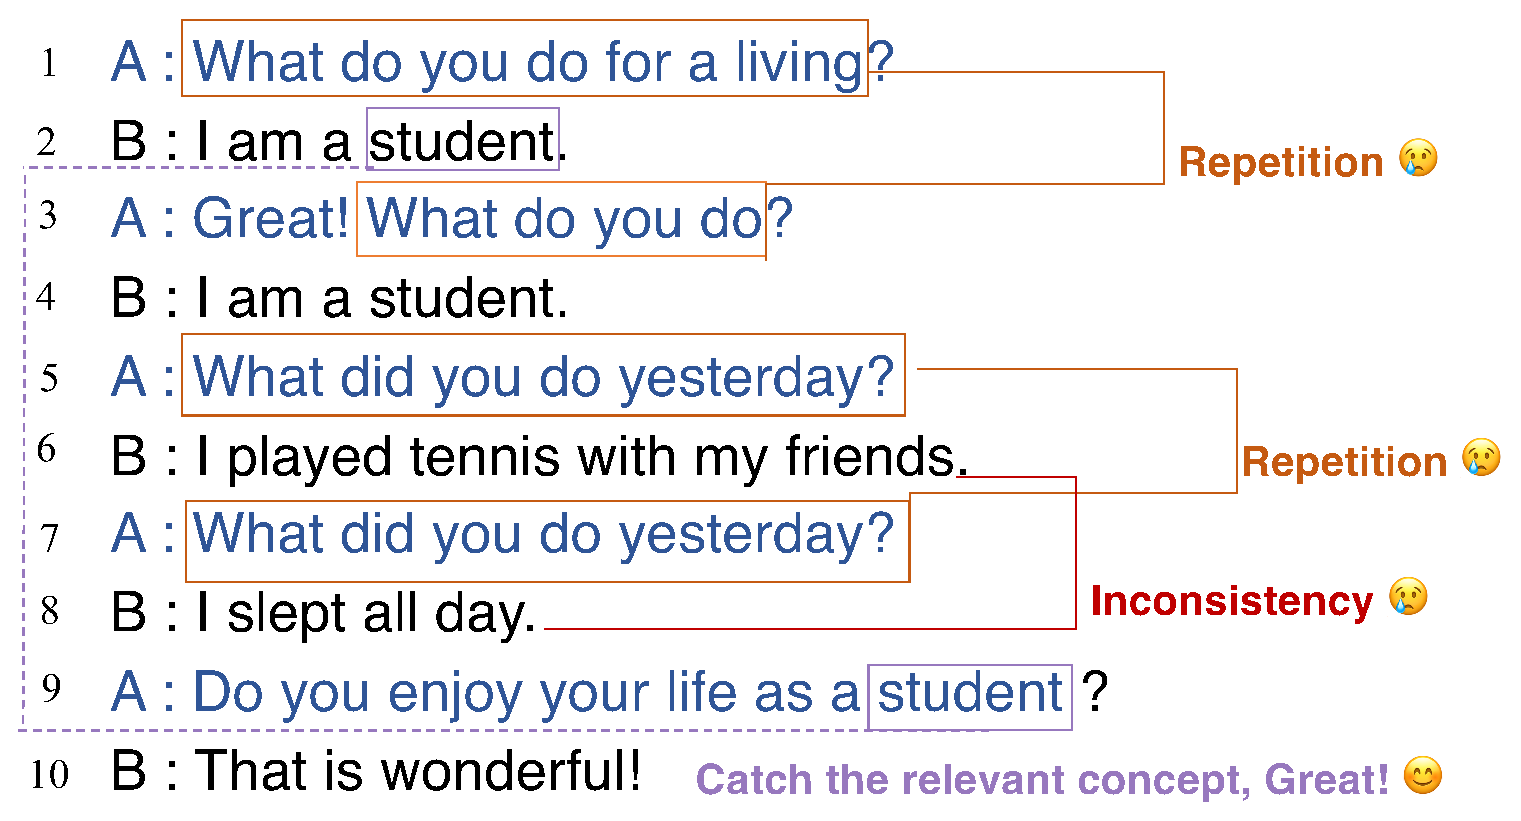
\includegraphics[width=0.95\columnwidth]{example2.eps}
        \caption{A chat snippet between two bots.}
        \label{fig:example}
\end{figure}

Fluency, Knowledge, Proactivity and Specificity are scored for each turn separately
and aggregated at the end of the conversation.
Detection for diversity, consistency and relevance are more involved and are explained
using \figref{fig:example}. 

As for diversity, at each turn $t$, we first check if there exists any repetitive question.  
We can easily find turn 3 and turn 7 repeated turn 1 and turn 5 
respectively. They will then be penalized one point for repetition. 
Repetition is not penalized if the previous turn is already 
marked as a repetitive question. For example, in \figref{fig:example}, 
although turn 4 is considered a repetition of turn 2,  
we are not going to penalize it as turn 3 is a repetitive question. 

The detection of inconsistency is always triggered after the detection of repeated questions. 
If the answers to the same questions are different, we will penalize the current turn, 
such as turn 8 in \figref{fig:example}.

We decide a repetition or an inconsistency by calculating the similarity of the two turns. 
We use a similarity function to complete the calculations, which we will 
discuss in \secref{sec:experiment}. The actual diversity and consistency scores
are the negation from the amount of repetition and inconsistency.

Relevance is assessed as a bonus to reward
a bot if it is able to memorize the important relevant concepts that have shown up 
before in the conversation. We sort the concepts that have shown up in 
chat history by their IDF scores. For example, in turn 9, $A$ 
mentions the concept word ``student'' presented by $B$ in turn 2. With this
turn, $A$ will win a bonus point.


The algorithms and notations for computing diviersty, consistency and relevance are included
in \tabref{tab:functions}, \algoref{algo:rep}, \algoref{algo:inconsist}, and \algoref{algo:bonus}. 

\begin{table}[th]
\centering
\small
\begin{tabular}{c|l}
%\hline
\toprule
\textbf{Notation} & \textbf{Description} \\ \midrule
$t$ & Current turn \\
$H(t)$  &  a list of history turns prior to $t$ \\
$Sim(x,y)$ & similarity between two turns $x$ and $y$ \\
$\sigma_r$ & Threshold for detecting repetition \\
$\sigma_c$ & Threshold for detecting consistency \\
$r$ & Weight for repetition \\
$c$ & Weight for inconsistency \\
$b$ & Weight for bonus \\
$d$ & Min distance between consecutive mentions \\
IDF list & List of lemma in chatlog sorted by IDF\\
$p$ & Percentage of important lemmas in IDF list\\
$R(t)$ &  Repetition penalty for turn $t$ \\
$C(t)$ &  Inconsistency penalty for turn $t$ \\ 
$B(t)$ &  Memory bonus for turn $t$ \\
$Rep(t)$ & A list of repeated turns for turn $t$ \\  
\bottomrule
\end{tabular}
\caption{
Functions and variables in algorithms.}
\label{tab:functions}
\end{table}

\begin{algorithm}[th]
\small
\caption{Scoring for Diversity}
\label{algo:rep}
\hspace*{0.02in} {\bf Input:}
 $t$, $H$, $Sim$, $\sigma_{r}$
; \hspace*{0.02in} {\bf Output: } 
 $R$;
\begin{algorithmic}[1]
\State //Starting to detect repetition
\For {$u$ in $H(t)$}
	\If {$Sim(t,u) \geq \sigma_{r}$}
		\State Add $u$ to $Rep(t)$
	\EndIf
\EndFor
    \If{$len(Rep(t))\geq 0$}
        \If{$t$ is a question and We can find a question in $Rep(t)$}
        \State $ R(t) \leftarrow  R(t) + 1$ 
        \Else
        \If {the previous turn of $t$ is not a repetitive question}
        \State $R(t)) \leftarrow R(t) + 1$ 
        \EndIf
        \EndIf
    \EndIf
\end{algorithmic}
\end{algorithm}


\begin{algorithm}[th]
\small
\caption{Scoring for Consistency}
\label{algo:inconsist}
\hspace*{0.02in} {\bf Input:}
$t$, $H$, $Sim$, $\sigma_{c}$
; \hspace*{0.02in} {\bf Output:  } 
 $C$;
\begin{algorithmic}[1]
\State // Inconsistency detection
 \If {previous turn of $p$ is a repetitive question} 
   \If{ the response $res$ to the question repeated by turn $p$ contradicts turn $i$ with $Sim(t, res) \leq \sigma_{c}$ }
    \State $C(t) \leftarrow C(t) + 1$
   \EndIf
  \EndIf
\end{algorithmic}
\end{algorithm}

\begin{algorithm}[th]
\small
\caption{Scoring for Relevance}
\label{algo:bonus}
\hspace*{0.02in} {\bf Input:}
$t$, $p$, $d$
; \hspace*{0.02in} {\bf Output:  } 
$B$;
\begin{algorithmic}[1]
\State // Assessing the ability of catching relevant concepts\\
$B(t) \leftarrow 0$
\For {all tokens $tk$ in current turn $t$}
 \If {$t$ - previous occurrence turn of $tk > d$ and $tk$ in the top $p\%$ of the IDF list of all tokens in the dialogue} 
   \State $B(t) \leftarrow 1$
  \EndIf
 \EndFor
\end{algorithmic}
\end{algorithm}

At the end of each game, each bot gets seven scores, one for each dimension.  
After pairwise comparison on individual dimension, a bot gains one point for win and zero point for a tie or lose.
The final score of each bot is determined by the sum of their individual scores.
%\KZ{Are these scores positive or negative? Comparable between bots?}

\subsubsection*{Match-level Scoring}
%\KZ{Use an equation to compute the final scores?}
One match which consists of two games, each started with a different bot, 
decides winning or losing between two bots.
For match-level scoring, we mimic the scoring rules of soccer tournament. 
For each match, $W$ points for the winner,  
$T$ points for a tie and 
$L$ points for the loser.
The value of $W$, $T$ and $L$ will be discussed in \secref{sec:ablation}. 

%\KZ{At the match level, we need to consider different starting context for the bots? I think we should present a few options for the reader and say that we are limited to these.}

\subsubsection*{Tournament-level Scoring}
%\KZ{Use an equation to compute the final scores?}
We count the points by simply summing up their scores gained in every match. Currently, several bots with the same final rank are tolerated. For future study, it's possible to mimic more detailed rules presented in sports match such as determine their ranking based on their win-loss relationship in the match between them.  
If they are still tied, we could propose an “overtime” for these two bots, one human judge may observe their performance and then make the decision of the game.


\subsection{Experimental Setup}
\label{sec:preprocess}
In this paper, we use Probase\cite{WuLWZ12} and WordNet\cite{wordnet}
as two alternative isA taxonomies. Probase is a large collection of
concept-subconcept or concept-entity pairs which were
extracted automatically by the Hearst pattern\cite{Hearst92} from
a large web corpus. Because this knowledge base is harnessed from large
data, it contains statistical scores of the extracted pairs,
such as the popularity,
and the conditional probability between the concept and its sub-concept.
WordNet, on the other hand, is a smaller, cleaner knowledge base manually
curated by experts and does not contain any scoring information.
These two taxonomies provide two different vocabularies of concepts
from which to draw the solution of AC.
%Our primary target of verb is a set of 200 most frequently used verbs in
%English text\footnote{We compute the frequency of all verbs that appeared
%in a very large web text corpus to obtain the 200 most frequently used
%verbs. We excluded a few verbs such as ``use'', ``make'', ``get'' and
%``take'' from the top of the list because they are extremely general and
%have too many arguments.},
%which we call Verb-200. These verbs are shown in \figref{fig:verbs}. A random
%sample of 20 verbs from Verb-200 forms a smaller set of verbs called Verb-20
%(highlighted in \figref{fig:verbs}) which are used in most of our experiments.

All our experiments are based on two large
datasets\footnote{We release most of
our datasets and the action concept lexicon at
\url{http://adapt.seiee.sjtu.edu.cn/~kzhu/ac}.}
from Web sentences (called Web for short) and
Google syntactic N-gram data\cite{goldberg2013,googlengram}
(called Google for short), respectively.
The 3734 most frequently used verbs (including verb phrases)
in the Web data form a primary verb set called {\bf Verb-3734}.
A subset of 2323 verbs that can be found in the Google dataset
form another verb set called {\bf Verb-2323}.
%We compute the frequency of all verbs that appeared
%in a very large web text corpus to obtain the 3734 most frequently used
%verbs.
A random sample of 20 verbs from the 200 most frequently
used verbs form the smallest set of verbs called {\bf Verb-20}
(in \figref{fig:verb20}), %which are used in most of our experiments.
which are used in some of the experiments.

The Web dataset contains 49,911,718 verb-subject pairs
and 65,035,827 verb-object pairs extracted from 165,758,215 English
sentences, which is a crawled snapshot of web pages.
%\KZ{How many subject-verb pairs and verb-object pairs in web data?}
%\KZ{How many?}\textcolor{red}{[KQ:We don't know...]}
%in a snapshot of Bing's search log.
The Google dataset contains
32,731,395 verb-subject pairs and 43,580,062 verb-object pairs
from the \emph{Verbargs} package, which includes 130,436,458
syntactic N-grams.% with verb-argument dependencies.
%\KZ{How many subject-verb pairs and verb-object pairs in google data?}
%\KZ{Kaiqi: We need to describe how we generate the web and
%google data sets here.
%Need to emphasize how big these data sets. Remember this ``VL''DB!}

\begin{figure}[th]
\centering
\fbox{\parbox{.8\columnwidth}{
bring,
carry,
connect,
cut,
define,
eat,
help,
hit,
keep,
operate,
perform,
play,
read,
release,
report,
select,
spend,
submit,
visit,
wear
}}
\caption{Verbs in Verb-20}
\label{fig:verb20}
\end{figure}

ReVerb also provides millions of relation triples, some of which contain
verbs as predicate.
%However, the scale of ReVerb is small to our problem.
We aim at discovering the action concepts,
which needs a large number of action instances
for each verb. However, ReVerb contains small number of triples for each verb.
For example, only 374 unique triples for ``wear'' are
extracted in ReVerb while our web dataset contains 17,749 unique
\pair{verb}{object} pairs for ``wear''.
The reason of the huge different is that,
a triple must contain two arguments for the verb in ReVerb. However,
verbs co-occur with only one argument in many cases.
Moreover, ReVerb has little coverage on
intransitive verbs, which only come with subject.
We give up using ReVerb data due to these limitations.
%\KZ{We need to explain why we don't use the ReVerb data.}

%\subsection{Preprocessing of Dataset}
%To make use of the web sentences and Google syntactic N-gram,
Next, we preprocess the two datasets as follows to
generate action instances.

{\bf Web} data comes from the result of Stanford dependency parser,
%We run a dependency parser on the whole corpus and
which are dependency trees for the sentences. We are interested in
verb-subject and verb-object relations only.
The head word of subject is usually labeled
as ``nsubj'' or ``agent'' while the head word of object is usually
labeled as ``dobj'' or ``nsubjpass''.
We can retrieve the entire phrase of subject or object in the dependency
tree by returning the whole subtree rooted on the head.
However, the whole phrase of subject/object is not always
a term recognizable by the taxonomies. As shown in \figref{fig:pterm},
the phrase ``a flashy baseball cap''
is extracted as the object of ``wear'', but 
it is not a valid Probase/WordNet term.
To make use of the taxonomies, we need to
detect the Probase/WordNet term from the subject/object phrase
(e.g., baseball cap).

\begin{figure}[th]
\centering
\epsfig{file=pterm.eps,width=0.8\columnwidth}
\caption{Dependency Parse Tree}
\label{fig:pterm}
\end{figure}

We use a sliding window strategy to extract longest
Probase/WordNet term that we can detect in the whole phrase.
The window slides around the head word
from right to left, and check if a Probase/WordNet term exists.
The initial size of the window is the length of the
whole phrase. If we detect a Probase/WordNet term,
we return the phrase captured in the window;
Otherwise, we decrease the window size and slides
around the head term again. We stop until we find
any Probase/WordNet term. Usually, this procedure can detect
a Probase/WordNet term from the phrase, because Probase/WordNet includes
most of the words (phrase with length 1). After
preprocessing, we output all the pairs of verb-subject and
verb-object as action instances.
%\begin{table}[th]
%\centering
%%\scriptsize
%\caption{Snapshot of Google Syntactic N-gram}
%\begin{tabular}{|l|l|}
%\hline
%Verb & N-gram \\
%\hline \hline
%accept & firms/NNS/nsubj/2\; accept/VBP/conj/0\; \\
%& money/NN/dobj/2\; in/IN/prep/2\; \\
%& exchange/NN/pobj/4   \\
%\hline
%delay & to/TO/aux/2\; delay/VB/xcomp/0\; \\
%& these/DT/det/4\; matters/NNS/dobj/2 \\
%\hline
%spent & an/DT/det/2\; afternoon/NN/nsubjpass/4\; \\
%& was/VBD/aux/4\; spent/VBN/conj/0\\
%\hline
%\end{tabular}
%\label{tab:ngram}
%\end{table}

\textbf{Google} data contains relations between
verbs and arguments.
%A snapshot
%of Google syntactic n-gram is shown in \tabref{tab:ngram}.
%The syntactic n-gram consist of the dependency parsing
%result conducted by Stanford parser.
Each token is labeled with POS tag, dependency and head index.
To apply this data to our task,
we restore each n-gram to a dependency tree according
to the head index and 
adopt the same processing as in Web to extract 
pairs of \pair{verb}{subject} and \pair{verb}{object}.
%First, we restore each n-gram to a dependency tree
%according to the head index. Next, we find the head of the
%subject or object from the nodes that directly connects to
%the verb node with a dependency label such as ``nsubj'', ``agent'', ``dobj''
%or ``nsubjpass''. Around the head, we use the same sliding window
%algorithm to find a longest Probase/WordNet term to be the subject/object
%as in the processing of the web data. Also, we convert
%the verb to its lemma form.
%After this process, we finally get two lists of pairs
%in the form of \pair{verb}{subject} and \pair{verb}{object}, respectively.

The subsequent experiments are conducted on lexicons learned from
different combinations of verb sets, taxonomies and datasets. For
readers' convenience, the configurations of these experiments are documented
in \tabref{tab:comb}.
\begin{table}[th]
\centering
%\scriptsize
\caption{Verbs, taxonomies and datasets for each experiment}
\begin{tabular}{|l|c|c|c|}
\hline
Experiment & Verb Sets & Taxonomies & Datasets \\
\hline \hline
Accuracy \& Overlap & Verb-20 & Probase &  Web, Google\\
\hline
\multirow{2}{*}{Execution Times} & Verb-3734, & Probase,
	& \multirow{2}{*}{Web, Google} \\
	& Verb-2323 & WordNet & \\
\hline
Verb Sense Matching & Verb-3734 & WordNet & Web \\
\hline
Argument Identification & Verb-20 & Probase & Web \\
\hline
WSD & Verb-3734 & WordNet & Web \\
\hline
Verb Frame Generation & Verb-3734 & Probase & Web \\
\hline
Term Similarity & Verb-3734 & Probase & Web \\
\hline
\end{tabular}
\label{tab:comb}
\end{table}

%\begin{figure}[th]
%\centering
%\fbox{\parbox{2\columnwidth}{
%\sout{use
%make
%include
%take
%get
%provide
%show}
%go
%say
%find
%see
%come
%work
%need
%look
%require
%give
%{\bf help}
%offer
%know
%create
%change
%add
%start
%allow
%{\bf keep}
%{\bf play}
%contain
%run
%apply
%receive
%call
%develop
%leave
%begin
%hold
%support
%cause
%build
%meet
%increase
%cover
%base
%want
%serve
%continue
%{\bf read}
%write
%produce
%{\bf bring}
%involve
%pay
%live
%ask
%put
%consider
%set
%reduce
%remove
%improve
%appear
%{\bf perform}
%seem
%move
%lead
%follow
%buy
%occur
%try
%design
%contact
%complete
%sell
%learn
%determine
%think
%{\bf report}
%describe
%like
%present
%mean
%relate
%lose
%feel
%affect
%post
%represent
%enjoy
%send
%open
%discuss
%{\bf visit}
%enter
%grow
%share
%maintain
%identify
%indicate
%tell
%place
%list
%return
%choose
%{\bf select}
%turn
%sign-up
%form
%obtain
%stop
%check
%result
%win
%happen
%install
%{\bf wear}
%die
%love
%understand
%save
%expect
%focus
%fill
%watch
%prevent
%{\bf spend}
%protect
%reach
%pass
%raise
%display
%treat
%ensure
%{\bf connect}
%achieve
%establish
%suggest
%view
%accept
%associate
%fit
%drive
%exist
%control
%talk
%replace
%deliver
%avoid
%hear
%fall
%let
%{\bf define}
%handle
%{\bf eat}
%plan
%bear
%prepare
%manage
%{\bf release}
%promote
%attend
%experience
%join
%kill
%seek
%{\bf operate}
%measure
%end
%refer
%teach
%face
%conduct
%explain
%purchase
%combine
%test
%{\bf cut}
%generate
%review
%deal
%break
%close
%reflect
%decide
%believe
%consist
%{\bf carry}
%fail
%collect
%speak
%address
%encourage
%match
%stand
%sit
%stay
%{\bf hit}
%{\bf submit}
%draw
%walk
%depend
%limit
%please
%reveal
%introduce
%wait
%arrive
%enable
%}}
%\caption{Verb-200 (Ranked) with Verb-20 in Bold}
%\label{fig:verbs}
%\end{figure}

%bring\\
%carry\\
%connect\\
%cut\\
%define\\
%eat\\
%help\\
%hit\\
%keep\\
%operate\\
%perform\\
%play\\
%read\\
%release\\
%report\\
%select\\
%spend\\
%submit\\
%visit\\
%wear\\
%\hline
%\end{tabular}
%\label{tab:verbs}
%\end{table}
%




\section{Methods}
\label{sec:method}
%In addition to FMB and AMB, we also provide a human baseline for the proposed task. We will introduce them in this section.
For textual QA pairs generation, a general method is the basic two-step framework consisting of answer extraction and question generation.
This will be the backbone of our method and we will first introduce this framework including the modules we used.

Then, in order to 
%effectively consider 
%the information of aspect keywords, 
generate the aspect related QA pairs from text,
we designed two methods: 
%In this section, we will introduce our methods to generate QA pairs related to aspect keywords, including
the Filtering Method and Aspect-based Method.
The former model is 
%naive and intuitive 
to use a filter to discard the irrelevant QA pairs, 
while the latter model considers effectively encoding the information of aspect keywords in the two-step framework.
%These two methods are  talk about the Filtering Method and Aspect-based Method.

\subsection{Two-step Generation Framework}
\label{sec:two-step}
%In this task, we aim at generating several QA pairs with an input paragraph $P$ and the aspect keyword $Aspect$.
A textual QA pairs generation task aims at generating several QA pairs with an input context.
The two-step generation framework is first extracting the answer from context and then generating questions based on the context and extractive answer.
%Next, we will introduce these two steps.
\subsubsection{Answer Extraction}
Same as most of other QA pairs generation methods, answers are first extracted to prepare for the subsequent question generation.
In this module, we choose two model to extract answers from context.
\paragraph{Chunking (Ck)}
\label{sec:chunk+nohint}
Subramanian et al.~\shortcite{subramanian2017neural} have extracted all of the named entities from the context as the answer candidates, then they use a classifier to identify whether a named entity can be considered as a reasonable answer.
The disadvantage of this approach is that not all of the answers are named entities, there are more answers in our data set cover the phrases with various meanings.
% such as noun phrases, preposition phrases, verb phrases, etc.
In the example shown as Figure \ref{fig:wiki}, the answer ``1908" is about time which is a named entity, the answer ``rats and fleas" is a noun phrase and ``the Justinian plague that was prevalent in the Eastern Roman Empire from 541 to 700 CE" is a clause.

In order to get the meaningful phrases as much as possible, we use the parser of Stanford CoreNLP~\cite{manning-EtAl:2014:P14-5} to find specific types of chunks such as noun phrases, preposition phrases, verb phrases, clauses, etc\footnote{We used all the phrase structure grammar representations provided by Stanford parser.}. 
%\SY{The types of phrases we choose are listed in Appendix A.}
Then we use a classifier to select the subset of extractive chunks which are suitable as answers.
It is fine tuned by BERT and takes the context (i.e., a sequence of words) and the words of answer as the input segments.
The input positive samples are the phrases exactly matched with human annotated answers provided in our dataset.

%\SY{ranking \& DP}
%For an answer $a_i$, we can obtain $P(a_i|Context)$ by BERT classifier then 
For extracting the best answers from a context, we expect to maximize $\sum^{n_a}P(a_i|Context)$ where $P(a_i|Context)$ is obtained by BERT classifier. 
Due to the high overlapping of the extracted answers, 
we use dynamic programming to schedule the weighted answer interval for deduplication:s
\begin{equation*}
\small
S(a_i) = \begin{cases}
0, i = 0\\
max(S(a_{i-1}, S(frt(i)+P(a_i|Context))))
\end{cases}
\end{equation*}
%where $A=\{a_1,a_2,...,a_|A|\}$ is the answer list selected by the classifier, $frt(i)$ 
, where $A=\{a_1,a_2,...,a_{|A|}\}$ is the list of answers obtained from the classifier and sorted in ascending order according to the ending position of the answers,
$frt(i)$ 
represents the non-overlapping answer nearest to $a_i$ in the list,
and $S(a_i)$ is the maximum probability sum obtained by the $i$-th answer.

%where Represents the previous compatible maximum working number in the sequence

\paragraph{Pointer Network (Ptr)}
Because pointer network works well on generating all possible answer positions from context~\cite{subramanian2017neural},
we also choose this as a method for answer extraction module.
The input of the model is a context (i.e., a sequence of words) and the output is a sequence of answer spans, which is formatted as $\{s_{a_1}, e_{a_1},s_{a_2}, e_{a_2},...,s_{a_1{|A|}}, e_{a_{|A|}}\}$.
$s$ and $e$ represent the start and end position of an answer respectively.

%Same as most of other QA-pair generation tasks, we extract answers from the document first.
%Follow the work of Subramanian et al.~\shortcite{subramanian2017neural}, we choose the pointer network to extract answers.
%The input is $(P_i, Aspect)$ pair from retrieval. For entity tagging, we use the spaCy\footnote{https://spacy.io/docs/usage/entity-recognition} to predict entities in $P_i$ and keep all entities. For the pointer network, it will generate all possible answer positions of $P_i$. We implement pointer network as Subramanian et al's~\shortcite{subramanian2017neural}.
\subsubsection{Question Generation (QG)}
After extracting answers from the context by last step, we can generate questions based on the context and corresponding answers.
%and the input tuple for this step is $(Context, a_i)$, where $a_i \in A=\{a_1, a_2,..., a_{|A|}\}$.
In this step, we choose UNILM model~\cite{dong2019unified} which is the SOTA method for Question Generation.
it realizes this task with the help of a language model which trained with the combination of uni-direction, bi-direction, and seq2seq.
Similar to the answer extraction step, for each tuple, 
we use ``[SEP]'' tokens to split the input segments.
%we combine the two segments in the same sequence as the first segment of UNILM and use ``[SEP]'' tokens to split the context and answer:
The input contains three segments: $Context, Answer$ and $Question$:
\begin{equation*}
\begin{aligned}
{Context [SEP] a_i [SEP] q_i}\\
\end{aligned}
\end{equation*}
where $a_i$ is an answer in $A=\{a_1, a_2,...,a_{|A|}\}$ extracted from context, $q_i$ is the target question for $a_i$. 
%And the second segment is the generated question.
\subsection{Filtering Method}
%%Filtering Method is divided into three steps: Answer Extraction, Question Generation and Filtering. 
%Filtering Method is 
%%With the two-stage method, 
%The first two steps can be unified into the two-step generation framework,
%and it is easily to generate several QA pairs with the input context.
Filtering Method is to add a filter module on the basis of two-step framework.
%To ensure that the generated QA pairs are aspect related, 
%an intuitive way is to 
%%train a filter to remove those irrelevant QA pairs.
%use a filter to make the judgment of whether the QA pair is relevant to the aspect keyword. 
%It is designed to make the judgment of whether a QA pair is relevant to the aspect keyword,
%and ensure that the generated QA pairs are aspect related.
After generating adequate QA pairs, 
a filter is designed to make the judgment of whether a QA pair is relevant to the aspect keyword
and remove the irrelevant ones.
%In this method, all steps are trained separately and following is the introduce about filtering.
%\paragraph{Answer Extraction.} Same as most of other QA-pair generation methods, we extract answers from the document first.
%
%Follow the work of Subramanian et al.~\shortcite{subramanian2017neural}, we use two methods, entity tagging (NER), and pointer network, to extract answers.
%The input is $(P_i, Aspect)$ pair from retrieval. For entity tagging, we use the spaCy\footnote{https://spacy.io/docs/usage/entity-recognition} to predict entities in $P_i$ and keep all entities. For the pointer network, it will generate all possible answer positions of $P_i$. We implement pointer network as Subramanian et al's~\shortcite{subramanian2017neural}.
%%Considering that the error of this step will continue to the next step,
%%while generating the question according to (paragraph, answer) pairs and generating the answer according to (paragraph, question) pairs are both hot research fields. 
%%we choose to generate answers first because we can extract answers from paragraphs instead of generating them, and extraction generally causes less error than a generation.
%
%We also tried the sequence labeling method. The BIO tagging model implemented by BiLSTM-CRF predicts ``O" for every token. We think the reason is the answer is too sparse in each $P_i$, which misleads the model to predict ``O'' for every token. So we split $P_i$ into sentences $\{S_{i,1}, S_{i,2}, ..., S_{i,n}\}$ and use tagging model to predict BIO tagging for each $S_{i,j}$. Finally, we combine all the sentence tagging as the tagging of $P_i$.

%\paragraph{Question Generation.} The input tuple for this step is $(P_i, A)$, where $A=\{a_1,a_2,...,a_m\}$ is the extracted answer list. We implement this based on two question generation models. One is seq2seq model~\cite{zhao2018paragraph}. This model uses RNN and gets self-attention to encode the paragraph and use another RNN to generate words sequence with copy mechanism. 
%
%Another one is UNILM model~\cite{dong2019unified}. UNILM is the SOTA method for Question Generation, it realizes this task with the help of a language model which trained with the combination of uni-direction, bi-direction, and seq2seq. Similar to the answer extraction step, for each input tuple, we combine the two segments in the same sequence as the first segment of UNILM and use ``[SEP]'' tokens to split paragraph and answer:
%
%\begin{equation*}
%\begin{aligned}
%{\rm P_i\ [SEP]\ a_i}\\
%\end{aligned}
%\end{equation*}
%where $a_i$ is an answer in $A$. And the second segment is the generated question.

\paragraph{The Filter}
%We get some QA pairs after the first two steps. In this step, we use a filter to make the judgment of whether the QA pair is relevant to the aspect. 
In order to identify the relevant QA pairs, we choose a binary sequence classifier as the filter. 
A filter takes the aspect, the answer and the question as the input and outputs a Boolean value as the judgment of whether the QA pair is relevant to the aspect. 
To make a better distinction between different segments of the input sequence, we add ``$[SEP]$'' tokens among different parts then the $i$-th input for a filter is ``$Aspect [SEP] a_i [SEP] q_i$''.

%We propose two strategies for model pretrain, one is context-based filter (CF) and another is QA-based filter (QAF).
%We propose one strategy for model pretrain, context-based filter.
%%The former way 
%It is based on the tree of Wikipedia pages and it regards the aspect keywords on the path to the context as the positive aspects, while the others are negative.
%In this case, there is difference between the input of training data formatted as ``$Aspect [SEP] Context$" and the target format of the filter, but all of the relevance labels are accurate.
%In the latter way, the data structure is consistent with the target, but the noise of training data is inevitable.
We propose one strategy for model pretrain,
it is based on the tree of Wikipedia pages.
If one aspect keyword is on the path to a context, it can constitute positive samples with the QA pairs of this context.
Conversely, the negative samples consist of aspect keywords and QA pairs that are not on the same path.
%  are  and regards the aspect keywords on the path to the context as the positive aspects, while the others are negative.
%In this case, there is difference between the input of training data formatted as ``$Aspect [SEP] Context$" and the target format of the filter, but all of the relevance labels are accurate.
In this case, the data structure is consistent with the target one, but the noise of training data is inevitable.

To ensure that the filter can learn reliable information of relevance between QA pairs and aspect keywords as well as reducing the impact of noise and differences of data, we use the annotated fine-tuning set to fine tune the filter model.

% In this part, we design a three-step pipeline structure which is shown as Figure \ref{fig:pipeline}. All steps are trained separately.

% %In this part, the answers are extracted from the source 
% \textbf{Paragraph Retrieval.} Two different methods are used here to select valid paragraphs with high relevance to the hint from the document.

% \textbf{Answer extraction.} Answers exist in the source document. The extraction module uses the approach of sequence labeling to mark the position of answers.

% \textbf{Question generation.} Question generation module is to generate questions from the document and a relevant answer span.

\subsection{Aspect-based Method}
%Same as the Filter Method, Aspect-based Method also has three steps: Answer Extraction, Question Generation, and Filtering.
The Aspect-based Method aims to effectively encode the information  of aspect in the two-step framework so that it can directly generate aspect related QA pairs.

%We don’t use Aspect information in answer extraction because the relevance between aspect and answers is not strong. 
To investigate whether the information of aspect keywords is helpful to two-step generation framework,
we randomly sampling 100 samples from the training data, 
finding only 34\% aspects are relevant to the answer. 
For example in the paragraph about Black Death:
\begin{equation*}
\begin{split}
&\text{Q : When did the plague return to Europe?} \\
&\text{A : throughout the 14th to 17th centuries} \\
&\text{Aspect : Recurrence}
\end{split}
\end{equation*}

The aspect is relevant to the QA pair but it’s not relevant to answer directly. Different from answer extraction, for more than half (about 56\%) of the samples, aspect keywords are directly relevant to the questions.
Thus, we only use aspects to help the model to generate more relevant questions.

For aspect-based question generation (QG$_{\text{Aspect}}$), we additionally encode the aspect keyword into the input of the source sequence and it is ``${Context [SEP] Aspect [SEP] a_i [SEP] q_i}$".
%\paragraph{Answer Extraction.} For methods mentioned in the Filter Method, we follow the same settings except that we use $P_i[SEP]Aspect$ to replace $P_i$ in the inputs. 
%
%One problem for the Filter Method is that it relies heavily on the accuracy of the filter. Based on this observation, we proposed a new method for Answer Extraction in the Aspect-based Method. In this new method, we first extract as many answer spans as possible and use a filter to omit some of them. This filter takes $(P_i, Aspect, Answer)$ triple as input and outputs whether the $Answer$ extracted from $P_i$ is related to the $Aspect$. We use a BERT classifier as the filter here. We made some adjustments to raise the threshold value of the triple to be determined as ``relevant'' to pass more QA pairs to the final filter.
%
%All samples will go through two filters in the process instead of only one. This gives our Aspect-based Method a better performance than the Filter Method.

%\paragraph{Question Generation. } 
%For the two proposed models in the Filter Method, we treat them differently. For the seq2seq model, to restrict the generated question with the aspect, we use another LSTM encoder for the aspect. Then use attention to aggregate information from aspect to the paragraph. The following equations shows the improved model.
%\begin{equation}
%\begin{aligned}
%u_{p} &= LSTM(e_{p}, m_{p}) \\
%u_{a} &= LSTM(e_{a}) \\
%u_{p} &= gated\ attention(u_{a}, u_{p})\\
%\end{aligned}
%\end{equation}
%Where $e_p$ and $e_a$ is the word embedding representation of  $P_i$ and $Aspect$. $m_p$ is the meta-word representation which identifies whether each word in the paragraph is in or outside the answer in $A$. The others are the same as the original model.

%For the UNILM model, we use the same method as Answer Extraction: replace all $P_i$ in the inputs with $P_i[SEP]Aspect$.

%\paragraph{The Filter. } We use the same filter as the Filter Method here. It takes the QA pair and $Aspect$ as input and output the relevance between these two inputs.
%In this method, we can still add a filter after the two-step framework to enhance the filtering ability of the model.

We can optionally add a filter to Aspect-based methods to enhance the filtering ability of the model.
It takes the QA pair and $Aspect$ as input and output the relevance between these two inputs.

%\subsection{Ranking Strategy}
%\label{sec:ranking}
%Both of the Filtering Method and Aspect-based Method can provide us a list of QA pairs for the given context.
%We expect the ranked QA pairs list is reasonable for a given aspect, so several ranking strategies are designed here.
%
%For the two-step framework using pointer network, the generated answer spans have equal probability because they are generated as a complete sequence. 
%Thus for the models with pointer network, we rank the generated QA pairs by the generative probability of each question $P(q_i|Context, a_i), a_i \in A=\{a_1, a_2,...,a_{|A|}\}$.
%The probabilities of questions can be calculated by the log-likelihood of the sequence with $N$ tokens, $N$ is the sequence length.
%
%For the two-step framework using chunking to extract answers, it is obvious that we can rank the generated QA pairs by $P(a_i|Context), a_i \in A=\{a_1, a_2,...,a_{|A|}\}$.
%The  probabilities of answers can be calculated by a binary classifier, that is, we take the ``$[CLS]$'' token into a linear layer of neural network and obtain the probability of the answer being positive.
%In addition, the score for the $i$-th QA pair can also be calculated as $P(a_i|Context) \times P(q_i|Context, a_i)$.
%To avoid the score of the product being 0, we normalized all probabilities to [0.1,1].
%
%In a word, we can get the ranked list of QA pairs by calculating the probability of generating the question ($\text{R}_\text{q}$), the probability of extracting the answer ($\text{R}_\text{a}$) and the product of the question and answer probabilities ($\text{R}_{\text{qa}}$) respectively.

%\subsection{Human Baseline} To measure the difficulty of each task, there were three master students to do each individual module in the pipeline method.
%For retrieval task, the students were asked to allocate the candidate paragraphs to 30 aspect keywords.
%For answer extraction, the students tried to extract answer spans  from 30 paragraphs.
%For question generation, they wrote the questions for 30 paragraphs with the given answers.
%The final scores of human performance were averaged.
%In this work, different ranking strategies to obtain the ranked list of QA pairs are based on the probability of extracted answers and generated questions.
%In this work, we obtain the probabilities of answers and questions from the binary

%The  probabilities of answers extracted by Chunking are calculated by a binary classifier, that is, we take the ``$[CLS]$'' token into a linear layer of neural network and obtain the probability of the answer being positive.




\section{Experiment}
In this section, we experiment on different NLG tasks. We first present the experimental setup on different tasks. Then, we show the quantitative and qualitative results together with comprehensive analysis and ablation studies.

\subsection{Implementation Details}
We evaluate the newly proposed ICL strategy on five commonly-researched natural language generation tasks: reading comprehension, dialogue summarization, style transfer, question generation and news summarization. Details on the task description, the strong baseline, corresponding  dataset, evaluation metrics and key hyper-parameters for each task are presented as follows.

\begin{table*}[th]
	\scriptsize
	\centering
	\begin{tabular}{lp{1.1cm}rrrcccc}
		\hline
		Task & Dataset & \#Train & \#Val & \#Test & Input & Output & Avg & Std\\
		\hline
		Reading Comprehension & DREAM & 6,116 & 2,040 & 2,041 & ``Q:''+ question + dialogue & answer & 5.59 & 2.61\\
		Dialogue Summarization & SAMSum & 14,732 & 818 & 819 & dialogue & summary  & 24.99 & 13.06\\
		Style Transfer & Shakespeare & 36,790 & 2,436 & 2,924 & original/modern  & modern/original  & 11.63 & 8.19 \\
		Question Generation & SQuAD1.1 & 75,722 & 10,570 & 11,877 & passage + [SEP] + answer & question & 13.09 & 4.27 \\
		News Summarization & CNNDM & 287,227& 13,368& 11,490 & document & summary & 70.97 & 29.59\\ 
		\hline
	\end{tabular}
	\caption{A summary of tasks and datasets. \#Train, \#Val and \#Test refers to the number of samples in the corresponding dataset. Avg and Std are the statistics for the number of output tokens. ``+'' refers to the concatenation operation.}
	\label{tab:taskdata}
\end{table*}

\textbf{Reading comprehension} is the task that answering questions about a piece of text. We use the DREAM dataset~\cite{sun2019dream} where questions are about corresponding dialogues and the answer is a complete sentence in natural language. We neglect the negative choices in the original dataset and formulate it as a NLG task. We adopt the pre-trained language model BART~\cite{lewis2020bart} as the baseline, where the input is a concatenation of a question and the corresponding dialogue made up of speakers and utterances. 
We experiment with  transformers\footnote{\url{https://github.com/huggingface/transformers}} based on the publically available ``facebook/bart-large'' checkpoint \footnote{\url{https://huggingface.co/facebook/bart-large}}.
%The preceding BART model is also adopted as the baseline, whereas the input is a concatenation of question and a dialogue.
The generated answers are evaluated by BLEU scores\footnote{The BLEU-1/2/3/4 scores are computed according the Google's implementation(\url{https://github.com/tensorflow/nmt/blob/master/nmt/scripts/bleu.py}).}~\cite{papineni2002bleu} widely used for QA systems, together with Meteor and Rouge-L F1 as mentioned above. The parameters are also the same as dialogue summarization, except that the early-stop is activated if there is no improvement on the perplexity of the validation set. 


\textbf{Dialogue summarization} is to generate a concise summary covering the salient information in the input dialogue. The preceding model BART has shown to be a strong baseline for this task, where only the dialogue is concatenated into a single sequence as the input. We experiment with  %transformers\footnote{\url{https://github.com/huggingface/transformers}} based on the publically available ``facebook/bart-large'' checkpoint \footnote{\url{https://huggingface.co/facebook/bart-large}} and 
SAMSum dataset\footnote{\url{https://arxiv.org/src/1911.12237v2/anc/corpus.7z}}~\cite{gliwa2019samsum} for daily-chat dialogues. 
The generated summaries are evaluated by comparing with the reference through evaluation metrics, including Rouge-1/2/L F1 scores\footnote{\url{https://github.com/pltrdy/files2rouge}}~\cite{lin2004rouge}, Meteor~\cite{banerjee2005meteor} and BertScore F1\footnote{Both Meteor and BertScore are calculated by SummEval(\url{https://github.com/Yale-LILY/SummEval}), and the latter one is based on the default bert-base-uncased model.}. We evaluate the model on the validation set after each training epoch and the early-stop patience will be added 1 if there is no improvement according to the Rouge-2 F1 score. The training process terminates when the early-stop patience equals or is larger than 3.  During the inference, the minimum and maximum output length is set to 5 and 100 respectively, with no\_repeat\_ngram\_size=3, length\_penalty=1.0 and num\_beams=4.


% The answer is either a span of words in the original text or a complete sentence in natural language.
\textbf{Style transfer} preserves the semantic meaning of a given sentence while modifies it's style, such as positive to negative, formal to informal, etc.
We adopt the Shakespeare author imitation dataset~\cite{xu2012paraphrasing}, containing William Shakespeare's original plays and corresponding modernized versions. Krishna el al.~\shortcite{krishna2020reformulating} proposed to do unsupervised style transfer by training paraphrase models based on the GPT-2 language model~\cite{radford2019language}. We re-implemented their approach STRAT\footnote{\url{https://github.com/martiansideofthemoon/style-transfer-paraphrase}} and evaluated with the provided script. Evaluation metrics includes 
transfer accuracy(ACC), semantic similarity(SIM), Fluency(FL) and two aggregation metrics, i.e., geometric averaging(GM) and their newly introduced $J(\cdot)$ metric. The hyper-parameter $hp$ equaling 0.0, 0.6 or 0.9  in Table~\ref{tab:end2endst} is the sampling parameter for trades off between ACC and SIM in their approach. 
In the training stage, we evaluate the model after updating every 500 steps. The perplexity on the validation set is used to activate the early-stop which equals 3. The inference is done as default.
 
\textbf{Question generation}~\cite{zhou2017neural} aims at generating a question given an input document and its corresponding answer span. SQuAD 1.1~\cite{rajpurkar2016squad} is generally used for evaluation. We adopt the data split as in \cite{du2017learning} and fine-tune the pre-trained UniLM~\cite{dong2019unified} as the strong baseline according to their official implementation\footnote{\url{https://github.com/microsoft/unilm/tree/master/unilm-v1}}. Generated questions are evaluated by metrics including BLEU-1/2/3/4, Meteor and Rouge-L with the provided scripts. The model is evaluated every 1000 steps and the early-stop equaling 3 is associated with the perplexity on the validation set. Other parameters are unchanged following the official guideline.

\textbf{News summarization} differs from dialogue summarization where the input is a document instead of a dialogue. We adopt the same strong baseline BART and evaluation metrics as dialogue summarization. Experiments are done with CNNDM dataset~\cite{HermannKGEKSB15} consisting of news articles and multi-sentence summaries\footnote{\url{https://github.com/pytorch/fairseq/blob/main/examples/bart/README.summarization.md}}. The model is evaluated every 2000 steps and the early-stop equaling 3 is associated with the Rouge-2 on the validation set. During the inference, the minimum and maximum output length is set to 45 and 140 respectively, with no\_repeat\_ngram\_size=3, length\_penalty=2.0 and num\_beams=4.
%\footnote{Inference parameters are borrowed from \url{https://github.com/pytorch/fairseq/blob/main/examples/bart/summarize.py}}

The summary of each task is listed in Table~\ref{tab:taskdata}. For fair comparisons, we re-implemented baselines following the above instructions on our machine. On top of the above baselines, we further arm them with the ICL strategy according to the Algorithm~\ref{alg:picl}. The settings of newly introduce Start and Stride are specified and discussed in following sub-sections. All of our experiments are done on a single RTX 3090 or a single RTX 2080Ti with 24G and 11G GPU memory respectively.
%and the result are averaged over three runs.


 
\subsection{Automatic Evaluations on Different Tasks}
\label{sec:taskperformances}

We compare our approach with the vanilla models mentioned above and the approach from~\citet{liang-etal-2021-token-wise} as baselines.
The performances on different NLG tasks are shown in Table~\ref{tab:end2end}. 
These tasks not only focus on solving different problems, but also has various amount of training data as well
as reference output lengths as shown
Table~\ref{tab:taskdata}.
Besides, the basic model are also different, including BART, GPT-2 and UniLM. 
Our new training strategy achieves significantly improvements among different tasks on most evaluation metrics, which shows that our method not only works well, but also has strong generalization abilities.

We explain the some specific results as follows:

(1) Our training strategy boosts the performances of the original STRAT with different $hp$ in the style transfer task. GM and J are two comprehensive evaluation metrics, with our approach topping the ranks with significant improvements.

(2) TCL generally performs poorly on tasks
with more training data. For example, it failed on question generation without any improvements over the vanilla model under the same parameter setting, while ICL still 
logs gains. This is mainly due to two reasons.
First, because the nature of TCL is data augmentation which is more effective in low-resource settings,
when training data is abundant, it becomes less useful. 
Second, the way they calculate the loss as sub-sequence generation better suites paraphrasing tasks, such as machine translation tested in their paper, as the order of 
the corresponding tokens between input and output 
are almost the same. Learning such forward mapping can 
be regarded as a kind of ``easy-to-hard'' 
in these limited scenarios.
However, this doesn't hold true for other tasks, 
such as summarization and question generation. 
Therefore, we didn't further test it on CNNDM since
CNNDM has the large amount of training data among
the five.

(3) For news summarization, Rouge-1 scores (precision, recall) for the baseline and our method on CNNDM are (38.16, 52.72) and (40.84, 49.23) correspondingly. Our method made substantial improvements on the precision with a compromise on the recall. 
The meteor score based on the unigram precision and recall emphasizes more on the recall than the Rouge-1 F1. As a result, it drops while Rouge-1 F1 increases. Overall, our method still outperforms BART on this task, especially on F1 scores of Rouge-2 and Rouge-L.




\begin{table}[th]
	\small
	\centering
	\begin{subtable}{\linewidth}
		\scriptsize
		\centering
		\begin{tabular}{lcccccc}
			\hline
			{Method} & {B1} & {B2} & {B3} & {B4} & {Met} & {RL}\\
			\hline
			w/o CL &  32.03 & 16.01 & 8.77 & \textbf{4.80} & 19.84 & 38.89\\
			TCL & 32.53 & 16.25 & 8.52 &4.67 &19.88 & 39.65 \\
			ICL &  \underline{\textbf{33.99}} & \underline{\textbf{17.43}} & \underline{\textbf{9.18 }}& 4.64 & \textbf{20.60} & \textbf{40.78}\\

			\hline
		\end{tabular}
		\caption{Reading Comprehension}
		\label{tab:end2endrc}
	\end{subtable}
	\\[5pt]
	\begin{subtable}{\linewidth}
		\scriptsize
		\centering
		\begin{tabular}{lccccc}
			\hline
			{Method} & {R1} & {R2} & {RL} & {Met} & {BertS} \\
			\hline
			%BART & 52.60&27.00 &42.10 &- & - \\
			w/o CL & 51.88 & 27.30 & 42.77 & 24.75 & 71.38 \\
			TCL  & 52.33 & 27.80 & \textbf{43.91} & 24.59 & 71.77 \\
			ICL & \underline{\textbf{53.07}} & \underline{\textbf{28.23}} & {43.83} & \underline{\textbf{26.12}}& \underline{\textbf{72.17}} \\
			
			\hline
		\end{tabular}
		\caption{Dialogue Summarization}
		\label{tab:end2endds}
	\end{subtable}
	\\[5pt]
	\begin{subtable}{\linewidth}
		\scriptsize
		\centering
		\begin{tabular}{lcccccc}
			
			\hline
			{Method}&$hp$ &  {ACC} & {SIM} & {FL} & {GM} & {J}\\
			\hline
			%\multirow{3}{*}{STRAT}& 0.0 & 71.70 & \textbf{56.40} & 85.20 & 70.10 & 34.70 \\
			%& 0.6 & 75.70 & 53.70 & 82.70 & 69.50 & 33.50 \\
			%& 0.9 & 79.80 & 47.60 & 71.70 & 64.80 & 27.50 \\
			%\hline
			\multirow{3}{*}{w/o CL}& 0.0 & 70.49 & 55.70 & 85.98 & 69.63& 33.72 \\
			& 0.6 &75.31 & 53.46 & 82.56 & 69.27& 33.30\\
			& 0.9 & 78.76 & 47.38 & 74.42 &65.24 & 27.88\\
						\hline
			\multirow{3}{*}{TCL } & 0.0 & 70.31 & \textbf{55.95} &\textbf{87.24} &  70.01& 34.71 \\
			& 0.6 & 74.79 & 53.14 & 82.56 & 68.97 & 33.21 \\
			& 0.9 & 79.41 & 46.88 & 71.92 &64.45 & 26.92 \\
			\hline
			\multirow{3}{*}{ICL}& 0.0 & \underline{73.72} & 55.91 & 86.30 & \underline{\textbf{70.60}} &\underline{\textbf{35.81}}\\
			& 0.6 & 77.26 & \underline{53.80} & \underline{83.87} & \underline{70.38} & 34.64\\
			& 0.9 & \textbf{79.65} & 48.16 & 76.06 & 66.32 & 29.03\\

			\hline
		\end{tabular}
		\caption{Style Transfer.}
		\label{tab:end2endst}
	\end{subtable}
	\\[5pt]
	\begin{subtable}{\linewidth}
		\scriptsize
		\centering
		\begin{tabular}{lcccccc}
			\hline
			{Method} & {B1} & {B2} & {B3} & {B4} & {Met} & {RL}\\
			\hline
			w/o CL & \textbf{50.38} & 35.67 & 27.24 & 21.36 & 24.40 & 50.67 \\
			TCL &\textbf{50.38} & 35.67 & 27.24 & 21.36 & 24.40 & 50.67\\
			ICL &  50.18 & \textbf{35.72} & \textbf{27.36} & \textbf{21.54} & \textbf{24.57} & \underline{\textbf{51.09}} \\
			\hline
		\end{tabular}
		\caption{Question Generation}
		\label{tab:end2endqg}
	\end{subtable}
		\\[5pt]
	\begin{subtable}{\linewidth}
		\scriptsize
		\centering
		\begin{tabular}{lccccc}
			\hline
			{Method} & {R1} & {R2} & {RL} & {Met} & {BertS}\\
			\hline
			%BART &  \\
			w/o CL &  43.07 & 20.01 & 35.94 & \textbf{21.44} & 63.72 \\
			TCL & - & -&- &- &- \\
			ICL & \textbf{43.39} & \underline{\textbf{20.55}} & \underline{\textbf{36.63}} & 19.68 & \textbf{64.05}\\
			\hline
		\end{tabular}
		\caption{News Summarization}
		\label{tab:end2endns}
	\end{subtable}
	\caption{Performances on different NLG tasks. ICL represents the models trained with our ICL algorithm. TCL refers to the previous work from~\cite{liang-etal-2021-token-wise}. Scores underlined are statistically significantly better than both re-implemented baselines with $p<0.05$ according to t-test. }	
	\label{tab:end2end}
\end{table}


\subsection{Human Evaluations}

To further prove the improvement of ICL, we hired three proficient English speakers for human evaluation. 20 samples from the test set of each task are randomly selected, ignoring the ones with totally same generations among three models, including the vanilla model, TCL and ICL. The original input, reference output and three generations are shown to annotators together, while the order of three generations are unknown and different among samples. 3-point Likert Scale is adopted for scoring for each generation~\cite{gliwa2019samsum}, where [1, 3, 5] represent 
excellent, moderate and disappointing results 
respectively. The average scores and agreements 
among the annotators are shown in 
Table~\ref{tab:humaneval}.

The Fleiss Kappa on the first four tasks indicates the fair to moderate agreements. It shows the promising improvement of ICL over the vanilla model and TCL especially on DREAM, SAMSum, and SQuAD1.1, which is consistent with the conclusion based on automatic metrics.
Although the agreement on style transfer is fair, 
our annotators without Shakespeare background 
tend to give low scores to all outputs.
Therefore, the absolute improvement is 
only $0.04$ compared to both baselines.
%This mainly due to the indistinguishable styles between
%Shakespeare’s plays with are quite different from modern languages. 
Besides, the poor agreement on CNNDM reflects the 
diverse concerns of summarization from different 
annotators. Without more specific instructions, they 
tends to focus more on the content coverage instead 
of checking the detailed facts. This is also 
consistent with the higher Meteor scores of the 
vanilla model over ICL.

\begin{table}[th]
	\scriptsize
	\centering
	\begin{tabular}{l|ccc|c}
		\hline
		{Datasets} & {w/o CL} & {TCL} & {ICL} & {Agreement}  \\
		\hline
		DREAM  &3.07 & 2.50&3.20 &0.48 \\
		SAMSum &2.97 &3.57 &3.97 &0.40 \\
		Shakespeare &2.23 &2.23 & 2.27&0.32 \\
		SQuAD1.1 &3.43 & 3.43 &3.77 &0.35 \\
		CNNDM & 3.45 &- &3.40 &0.11 \\
	%	\hline
	%	overall & & & &\\
		\hline
	\end{tabular}
	\caption{Human evaluations. The agreement is calculated by Fleiss Kappa.}
	\label{tab:humaneval}
\end{table}




%Following Liu et al.\shortcite{liu2021competence}'s work, we asked annotators to comparing the performance between our generated results and baselines by choosing from ``Better, Tie, Worse''. 
%The counts for each choice are shown in Table~\cite{}, where the Fleiss Kappa among annotators is ??.

%Analysis





%\subsection{Analysis on Variable Generation Lengths}

%Teacher forcing, which predicts each token given the reference summary tokens during training and given the previous generated tokens during inference, leads to the exposure bias problem for NLG tasks.
%Since ICL starts the training process by predicting the last few tokens of outputs and gradually calculates the loss based on more tokens when the model is stronger, we hypothesis that it can alleviate the exposure bias for training Seq2Seq models to some extent.
%As stated in~\cite{pang2020text}, the output quality tends to degrade as the output length increase with the exposure bias.
%So, we divided the test set of each task according to the length of the generated output into 4 buckets and randomly picked 20 samples in each buckets for both the corresponding baselines and our approach. Each generation is annotated by 5 point Likert Scale, where 1 is the worst and 5 is the best. 

%The trends of performances on variable generation lengths are in Figure~\ref{}.



\section{Results}
\label{sec:res}
In this section, we will discuss the results obtained by classification and word-pair difficulty ranking, 
%including the performance on various features and comparisons between baseline models and our feature engineering model.
including the comparisons between baseline models and our multi-faceted features model and the ablation tests for feature selection.

\subsection{Baseline Models}
In this section, we introduce the design of baseline models for the contrast experiments on classification and word-pair ranking tasks.
\subsubsection{Human Baseline}
To observe the limitation of human on classifying the word difficulty levels, 5 experts with educational background in foreign languages are chosen to do the classification task and word-pair difficulty ranking task respectively.
For classification task, each person was pre-trained with several words randomly selected from the standard difficulty levels, and were asked to allocate the difficulty levels for  100 words according to their learning outcomes and previous knowledge.
%In order to follow the actual distribution of word levels, the words to be labeled have the same distribution.
For difficulty ranking task, each person was given 100 pairs of words to label the difficulty relation of each pair. 
The words to classify and the word pairs are randomly sampled from the word list with the same distribution.
%Then we calculate the inter-judge agreement using Cohen's Kappa measurement. 

\subsubsection{Random Baseline (Random)}
In classification task, we follow the original distribution of word levels and randomly assign a level for each word and calculate the average accuracy of 10 runs.
In difficulty ranking task, 
each word pair will be randomly assigned with a difficulty relation.
%each word will be randomly assigned with a word in difficulty level to make up a word pair.
Then the accuracy will be calculated as the average of 10 runs.

\subsubsection{Frequency-Only Baseline (FO)}
%Frequency is a means of estimating the word difficulty. 
%As mentioned before, word difficulty has negative correlation with its frequency.
Frequency is a considerable feature on estimating the word difficulty.
%Some research discussed the correlation between word frequency and word difficulty, finding they are highly correlated~\cite{breland1996word}.
%There also exist some websites estimating the word difficulty based on word frequency\footnote{\url{https://www.twinword.com/api/language-scoring.php}}.
To construct the frequency-only baseline model, 
we calculate the word frequencies 
%of an open frequency dataset and a single corpus used in our experiment.
%\textbf{Frequency-only model based on the open dataset (FOMO)} calculates the English words' frequencies from SUBTLEX-UK list~\cite{van2014subtlex} and the  German words' frequencies from SUBTLEX-DE list~\cite{Bryant2011}.
%\textbf{Frequency-only model based on single corpus (FOMS)} calculates word frequencies 
based on different $Corpus$ mentioned in Section \ref{sec:data}.
The approach to construct the dataset for both classification and ranking tasks are the same as previous. 

%The open frequency list here means the SUBTLEX-UK list~\cite{van2014subtlex} for English or SUBTLEX-DE list~\cite{Bryant2011} for German.
%The words of SUBTLEX lists are both collected from subtitles of television programs, ordered by their frequencies.
%The single corpus used in our experiment is E1, E2 or G1 mentioned in Section \ref{sec:exper}.

\subsubsection{Frequency-Clustering Baseline (FC)}
Xiaobin Chen \shortcite{chen2016characterizing} implemented text readability classification by calculating mean frequencies of words from vocabulary bands and clusters respectively.
In this paper, we apply the clustering method to divide the vocabulary frequency bands.
%Intuitively, the distance between two words is the difference between their frequencies, so k-means is used for cluster analysis.
Intuitively, the Euclidean distance between each two words can be regarded as the difference on their frequencies:
$dist(w_i, w_j)=|Freq_{w_i}-Freq_{w_j}|$, then
we use K-means to do the clustering.
%As expected, the results of the cluster are consistent with the word frequencies distribution.
%The results of the clustering are consistent with the frequency distribution of words.
%The clustering results on The New York Times (E1) are shown as Figure \ref{fig:cluster}.
%It's clear that the frequencies bands can be  obviously divided by clustering.
Similarly, this baseline is also implemented on different $Corpus$ and different tasks.
%\SY{reviewer 2: There is no obvious clustering here.}

%\begin{figure}[th]
%	\centering
%	%	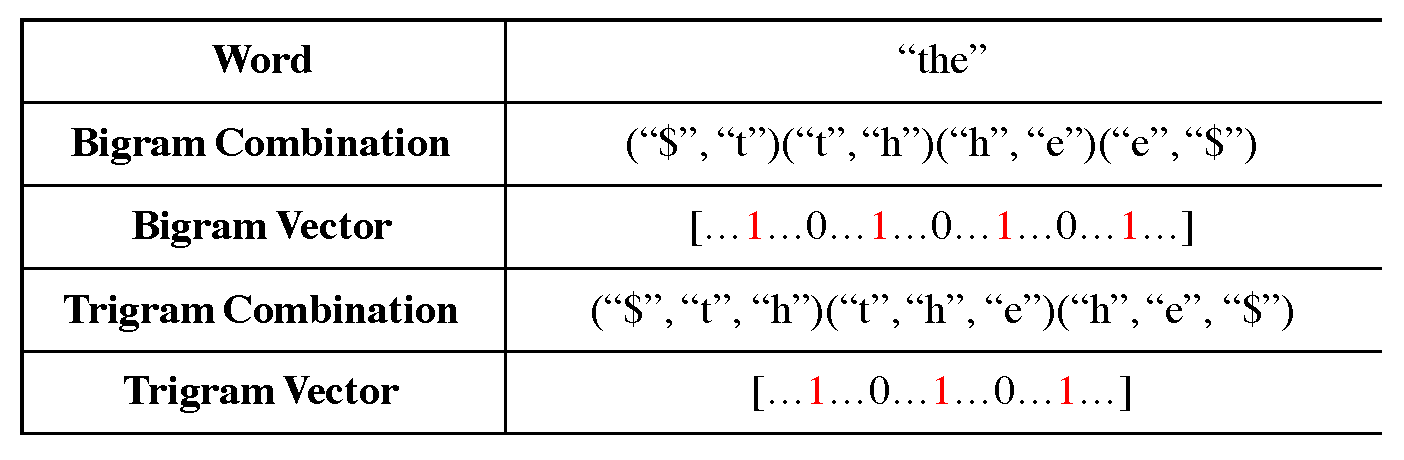
\epsfig{file=pic/bitri.eps, width=0.9\columnwidth}
%	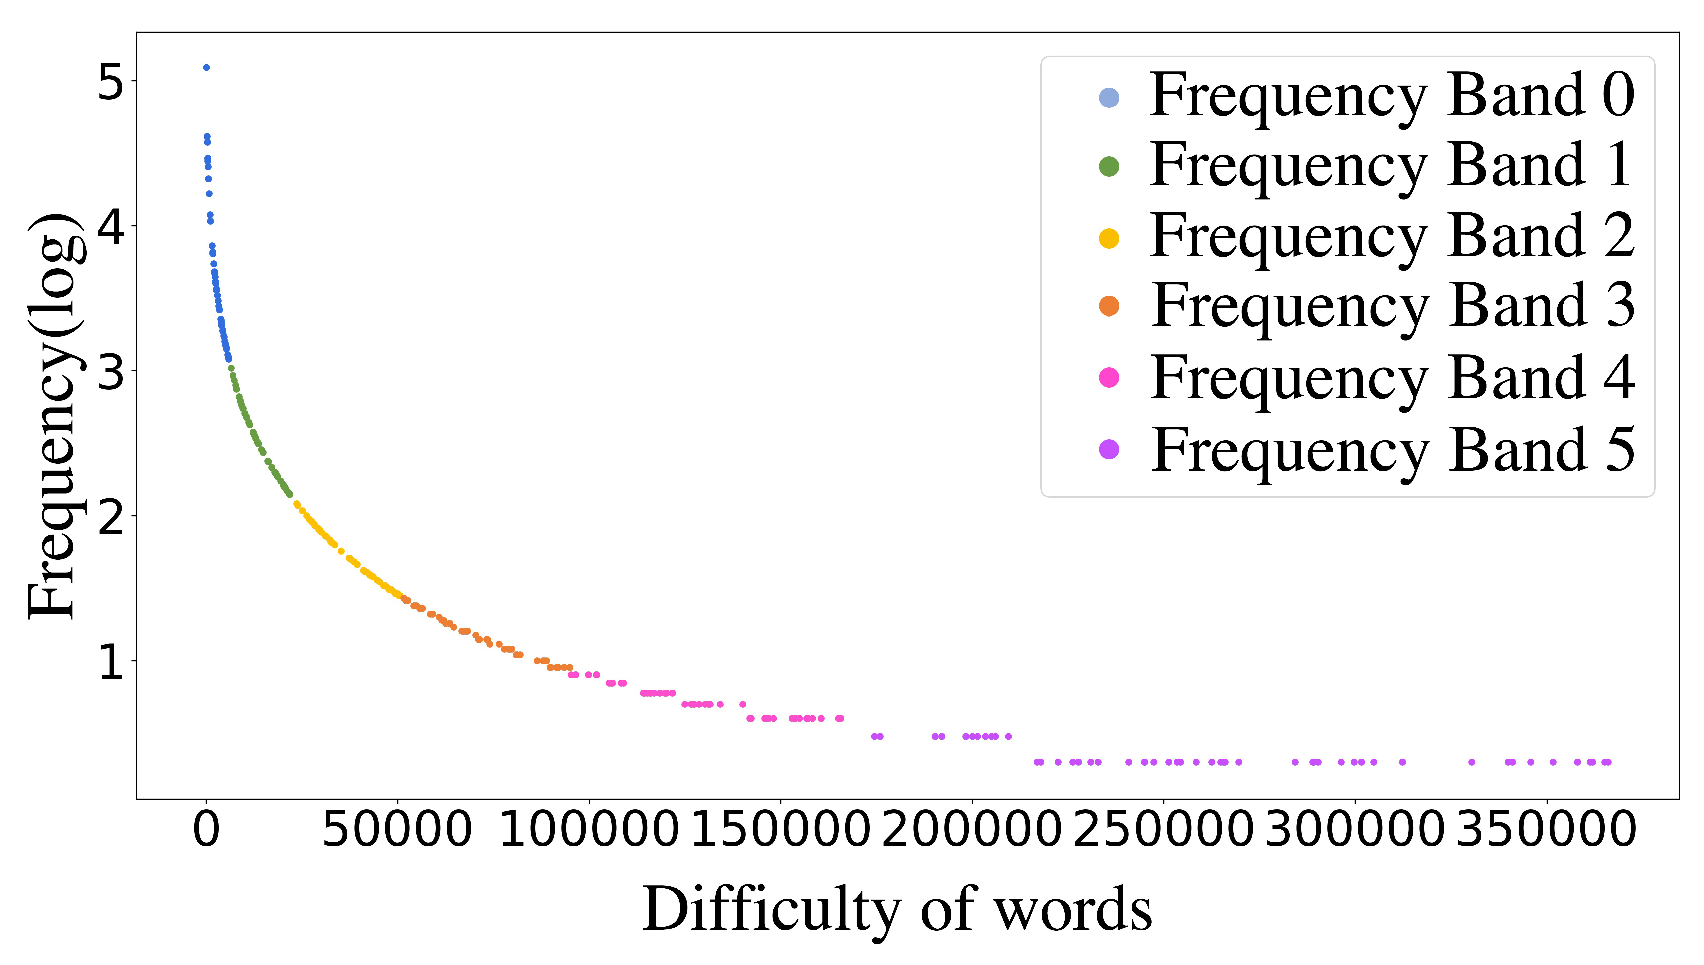
\includegraphics[width=1\linewidth]{pic/cluster.eps} 
%	\caption{Frequencies bands divided by clustering of the New York Times. The horizontal axis is the ranking of words ordered by difficulty, and the vertical axis is the log value of frequency.}
%	\label{fig:cluster}
%\end{figure}

%\textbf{FC Model based on the open frequency datasets (FCMO)} is implemented on English and German SUBTLEX lists.

%\textbf{FC Model based on the single corpus (FCMS)} is implemented on E1, E2 and G1 respectively.

%However, it can only achieve the accuracy of 8.91  of in English and the accuracy of 30.14  in German by predicting the word difficulty level by dividing the frequency of words into words.
%Once again proved that the difficulty of some words is not estimated completely by its frequency.
\subsubsection{Multi-Features Baseline}
%Several related studies in the fields of education and linguistics have mentioned that the compound of word frequency, length, the number of syllables in a word and the number of consonant clusters in a word~\cite{koirala2015word} and the compound of word frequency and POS tag~\cite{hiebert2019analysis} can be the features to measure word difficulty.
Several related studies in the field of education and linguistics combine features to do their tasks. 
The combination of frequency, length, syllables and phonemes and the number of consonant clusters is used in Koirala and Culligan's work~\shortcite{koirala2015word,culligan2015comparison}. 
Hiebert et al.~\shortcite{hiebert2019analysis} used word frequency and POS tags together to measure word difficulty.
Following these studies, we conduct the \textbf{FLSCP} (Freq+Length+\#Syllables+\#Consonant+\#Phonemes) baseline and \textbf{FPOS} (Frequency+POS) baseline.
%We also build \textbf{FLSCPV} (Freq+Length+\#Syllables+\#Consonant+Phoneme Binary Vector) which replaces the number of phonemes with the phoneme binary indication vector mentioned in Section \ref{sec:approach} to give a more fair and comprehensive comparison. 
Since these studies are only theoretical research and lack of automatic classification experiments, 
we use MLP to do the classification and ranking tasks based on these compound features.

\subsection{Results for Multi-faceted Features}
\label{sec:mmf}
%In this part, we discuss the results of our feature engineering method and other baseline models.
%The experiment is conducted on E1, E2, E1+E2 and G1.
%According to the result of the multi-class classification and difficulty ranking tasks shown in Table \ref{tab:resultsEnglish} and Table \ref{tab:resultsGerman}, we can draw the conclusion as follows.
The results of word difficulty classification and word-pair difficulty ranking tasks are shown in Table \ref{tab:resultsEnglish} and Table \ref{tab:resultsGerman} for different languages.
\textbf{MMF} represents the Multi-faceted Features mentioned in Section \ref{sec:approach}.
\begin{table*}[h]
	\scriptsize
	\setlength{\abovecaptionskip}{0pt}
	\setlength{\belowcaptionskip}{0pt}
	\begin{center}
		\begin{tabular}{lcccccccccccc}
			\toprule[1pt]
			& \multicolumn{4}{c}{\textbf{\begin{tabular}[c]{@{}c@{}}NY Times\end{tabular}}} & \multicolumn{4}{c}{\textbf{\begin{tabular}[c]{@{}c@{}} Gutenberg\end{tabular}}} & \multicolumn{4}{c}{\textbf{NY Times+Gutenberg}} \\ 
			\midrule
			& \multicolumn{2}{c}{\textbf{Classification}} & \multicolumn{2}{c}{\textbf{Ranking}} & \multicolumn{2}{c}{\textbf{Classification}} & \multicolumn{2}{c}{\textbf{Ranking}} & \multicolumn{2}{c}{\textbf{Classification}} & \multicolumn{2}{c}{\textbf{Ranking}} \\ 
			\midrule
			& \multicolumn{1}{c}{\textbf{Test}} & \multicolumn{1}{c}{\textbf{\textbf{CV}}} & \multicolumn{1}{c}{\textbf{Test}} & \multicolumn{1}{c}{\textbf{CV}} & \multicolumn{1}{c}{\textbf{Test}} & \multicolumn{1}{c}{\textbf{\textbf{\textbf{CV}}}} & \multicolumn{1}{c}{\textbf{Test}} & \multicolumn{1}{c}{\textbf{CV}} & \multicolumn{1}{c}{\textbf{Test}} & \multicolumn{1}{c}{\textbf{CV}} & \multicolumn{1}{c}{\textbf{Test}} & \multicolumn{1}{c}{\textbf{CV}} \\ 
			\midrule
			\textbf{Random}&20.57 &20.57 &49.85 &49.85 &20.57 &20.57 &49.85 &49.85 &20.57 &20.57 &49.85 &49.85 \\
			\textbf{FC}&8.23&8.23&67.50&67.50&17.53&17.53&30.36 &30.36 &22.41 &22.41 &55.00 &55.00 \\
			\textbf{FO}&34.20 &33.55 &66.10 &64.23&27.94&29.26&55.13 &57.56 &26.91 &28.23 &51.92 &53.22 \\
			\textbf{FPOS}&33.18&33.47&52.06&64.14&29.14&29.14&52.55&56.93&28.19&29.28&54.87&57.41 \\
			\textbf{FLSCP}&33.78&34.45&68.49&66.22&28.70&29.13&62.06&59.69&26.56&28.38&60.56&58.87\\
			\midrule
			%			[Fix+Word2Vec]+SVM&40.84 &39.59 &75.59 &78.77 &41.07 &36.36 &73.63 &74.31 &43.85 &39.32 &70.89 &65.74 \\
			\textbf{MFF+SVM$^{***}$}& 40.84& \textbf{39.59} & \textbf{75.59} & \textbf{78.77}& 41.07& \textbf{36.36} & 73.63 & \textbf{74.31} & \textbf{43.85} & \textbf{39.32}& 70.89& 65.74\\ 
			\textbf{MFF+MLP$^{***}$}&\textbf{42.94}&37.62&74.91&72.13&\textbf{41.18}&34.45&\textbf{74.88}&68.68&42.83&36.65&\textbf{76.29}&\textbf{72.76}\\
			%			[Fix+GloVe]+SVM&38.75 &36.56 &68.54 &65.43 &37.12 &36.25 &64.88 &62.05 &38.98 &36 &67.62 &63.48 \\
			%			[Fix+BERT]+SVM&41.76 &39.52 &74.15 &77.95 &42.46 &40.52 &73.5 &78.29 &43.85 &40.83 &71.93 &79.46 \\
%			\textbf{Fix+BERT}&42.11 &36.93 &68.55 &67.58 &\textbf{41.76 }&\textbf{35.78 }&64.19 &\textbf{69.12 }&\textbf{43.23 }&\textbf{38.92 }&65.48 &70.26 \\
%			\textbf{Fix+GloVe}&36.80 &34.97 &67.01 &67.35 &38.77 &34.86 &62.70 &68.22 &38.68 &35.15 &66.29 &69.72 \\
			\midrule
			\textbf{Human baseline}&49.28 &-&88.89 &-&49.28 &-&88.89 &-&49.28 &-&88.89 &-\\
			\bottomrule[1pt]
		\end{tabular}
	\end{center}
	\caption{\label{tab:resultsEnglish} 
		The classification and ranking results 
		%		 of different baseline models and our feature engineering methods by averaging ten runs 
		using two English $Corpus$ and their combination to extract the features.
		The accuracy for baseline models and our feature engineering models is the average of ten runs.
		\textbf{Test} means the accuracy on test set and \textbf{CV} means the accuracy on cross validation.
		\textbf{MFF} is the multi-faceted features using Word2Vec to obtain word embeddings.
		(*** indicates $p$-$value$ $<0.01$ compared with Random, FC, FO, FPOS and FLSCP baselines.)}
\end{table*}

\begin{table}[ht]
	\scriptsize
	\setlength{\abovecaptionskip}{0pt}
	\setlength{\belowcaptionskip}{0pt}
	\begin{center}
		\begin{tabular}{lcccccccc}
			\toprule[1pt]
			& \multicolumn{4}{c}{\textbf{\begin{tabular}[c]{@{}c@{}}Parallel Corpus for German\end{tabular}}} & \multicolumn{4}{c}{\textbf{\begin{tabular}[c]{@{}c@{}}Wikipedia for Chinese\end{tabular}}}\\ 
			\midrule
			& \multicolumn{2}{c}{\textbf{Classification}} & \multicolumn{2}{c}{\textbf{Ranking}} & \multicolumn{2}{c}{\textbf{Classification}} & \multicolumn{2}{c}{\textbf{Ranking}}\\ 
			\midrule
			& \multicolumn{1}{c}{\textbf{Test}} & \multicolumn{1}{c}{\textbf{CV}} & \multicolumn{1}{c}{\textbf{Test}} & \multicolumn{1}{c}{\textbf{CV}} & \multicolumn{1}{c}{\textbf{Test}} & \multicolumn{1}{c}{\textbf{CV}} & \multicolumn{1}{c}{\textbf{Test}} & \multicolumn{1}{c}{\textbf{CV}}\\ 
			\midrule
			\textbf{Random}&33.61 &33.61 &47.14 &47.14  & 16.63 &16.63 &43.03&43.03\\
			\textbf{FC}&34.93 &34.93 &49.24 &49.24 & 33.84 &33.84 &40.87	&40.87\\
			\textbf{FO}&36.83 &36.87 &53.42 &48.49 &54.02&	52.68&	62.99&	64.75\\
			\textbf{FPOS}&37.69 &36.77 &50.88 &48.44 &53.34	&53.17	&63.61	&65.90\\
			\textbf{FLSCP}&39.22 &37.46 &52.07 &53.67 &55.16&	53.77	&67.26	&66.60\\
			\midrule
			%			[Fix+Word2Vec]+SVM&42.39 &42.46 &70.47 &64.23 \\
			\textbf{MMF+SVM}&42.39$^{***}$	& 42.46$^{***}$ & \textbf{70.47$^{***}$}	& \textbf{64.23$^{***}$} & \textbf{57.80$^{***}$}	&54.95$^{***}$	&67.51$^{**}$	&\textbf{76.35$^{***}$}\\
			\textbf{MMF+MLP}&\textbf{47.74$^{***}$}&\textbf{42.50$^{***}$}&67.91$^{***}$ & 63.45$^{***}$  &56.96$^{***}$	&\textbf{55.84$^{***}$}	&\textbf{68.52$^{**}$}	&65.90$^{*}$\\
			%			[Fix+GloVe]+SVM &41.98 &42.42 &69.07 &65.74 \\
			%			[Fix+BERT]+SVM &42.39 &37.28 &52.88 &64.05 \\
%			\textbf{Fix+BERT}&46.30 &38.98 &54.14 &63.32 \\
%			\textbf{Fix+GloVe}&46.91 &41.73 &67.51 &69.14 \\
			\midrule
			\textbf{Human baseline}&44.44 &-&65.85 &-&&-&&-\\
			\bottomrule[1pt]
		\end{tabular}
	\end{center}
	\caption{\label{tab:resultsGerman} 
		The classification and ranking results using German and Chinese $Corpus$ to extract features.
		(*** indicates $p$-$value$ $<0.01$ compared with Random, FC, FO, FPOS and FLSCP baselines;
		** indicates $p$-$value$ $<0.01$ compared with Random, FC, FO and FPOS baselines;
		* indicates $p$-$value$ $<0.01$ compared with Random and FC baselines.)
%		The accuracy for baseline models and our feature engineering models is the average of ten runs.
%		\textbf{Test} means the accuracy on test set and \textbf{CV} means the accuracy on cross validation.
%		\textbf{Fix} is the compound features mentioned in this paper except word embedding.
		}
\end{table}
	
%	The explanation for this phenomenon is that FO focuses on word frequency itself and FC focuses on the frequency distribution of all words. 
%	There are more words in Gutenberg dataset which provides strong support to FC.
%	However a considerable part of words are older than those in New York Times, and this is the reason why it doesn't perform well on FOMS.

Comparing the results of baseline models for English such as FO, FC, FPOS, FLSCP and FLSCPV under NyTimes, Gutenberg and NyTimes+Gutenberg,
we find that the accuracy on both tasks varies substantially across different corpora.
%	Combined with the results in Section \ref{\textbf{sec:embedding}}, frequency is the best in the performance of the classification compared with length, POS and .
One possible explanation is that the large disparity in word frequency distribution leads to the unstable classification results among corpora. 
We found the P-value is less than 0.001 between the word frequency distribution of 
NyTimes and Gutenberg, which indicates there exists a significant difference.
%Thus, one possible explanation for the results is that the large disparity in word frequency distribution leads to the unstable classification results. 
Besides, 8 of the words in test set is correctly classified with features extracted under NyTimes while wrongly classified under Gutenberg and NyTimes+Gutenberg, which also supports the above conjecture.

Compared with the baselines, our proposed model takes more features 
into consideration, especially the syntactic and semantic features.
In Table \ref{tab:resultsEnglish}, we find that the results for both tasks are similar under different corpora and different classifiers, 
which are shown in the rows titled \textbf{MFF+SVM} and \textbf{MFF+MLP}.
The results in these two rows are significantly better than the baselines by T-test with $p$-$value$ $<0.01$.
Applied to different languages such as German and Chinese, the results of \textbf{MFF+SVM} and \textbf{MFF+MLP} in Table \ref{tab:resultsGerman} still have better performances than baselines.
Although frequency plays an important role in Chinese, the result also shows the superiority of multi-faceted features. 
The performance on three languages indicates that multi-faceted features 
is essential and effective for word difficulty classification.
It is also relatively stable among different language environments, showing a strong generalization ability which can 
be used in diverse language environments.
	
%Our proposed feature engineering model achieves the best results compared with previous models and it can achieve around 45  on classification task and 75  on ranking task.
%Overall, all the compound features with various embeddings on different corpus environments have shown to be significantly better than the previous state-of-the-art methods by T-test with p$<$0.01.

%From some prediction results of FO and ALL in Table \ref{tab:com}, we find our model can put some easy words into the correct level.
%Considering the words that are wrongly predicted by FO while correctly predicted by Fix+Word2Vec, Table \ref{tab:com} lists some examples to show our model is more inclined to classify the easier ones correctly.
%\begin{table}[th]
%	\scriptsize
%	\begin{center}
%		\begin{tabular}{ccccc}
%			\hline
%			\textbf{Word} & \textbf{Frequency in E1} & \textbf{FO} & \textbf{ALL} & \textbf{True Label} \\ \hline
%			weekday & 553 (9575/368939)& 6 & \textbf{2}& 2\\ 
%			pin & 1595  (4824/368936)& 6 & \textbf{3}& 3\\ 
%			birthday & 3507  (2728/368936)& 4 & \textbf{1}&  1\\ 
%			coffee & 5325  (2001/368939)& 4 & \textbf{1}& 1\\ 
%			\hline
%		\end{tabular}
%	\vspace{-0.25cm}
%	\end{center}
%	\caption{\label{tab:com} Prediction results of FO and Fix+Word2Vec.}
%\end{table}

%\begin{table}[th]
%	\scriptsize
%	\begin{center}
%		\begin{tabular}{ccccc}
%			\hline
%			\textbf{Word} & \textbf{Frequency in E1} & \textbf{FO} & \textbf{ALL} & \textbf{True Label} \\ \hline
%			weekday & 553 (9575/368939)& C2 & \textbf{A2}& A2\\ 
%			pin & 1595  (4824/368936)& C2 & \textbf{B1}& B1\\ 
%			birthday & 3507  (2728/368936)& B2 & \textbf{A1}&  A1\\ 
%			coffee & 5325  (2001/368939)& B2 & \textbf{A1}& A1\\ 
%			\hline
%		\end{tabular}
%	\end{center}
%	\caption{\label{tab:com} Prediction results of FO and Fix+Word2Vec.}
%\end{table}
%
% As for the words that are wrongly predicted by both FO and Fix+Word2Vec, Figure \ref{fig:distance} shows the distribution of their prediction labels and the ground truth.
%\begin{figure}[th]
%	\centering
%	%	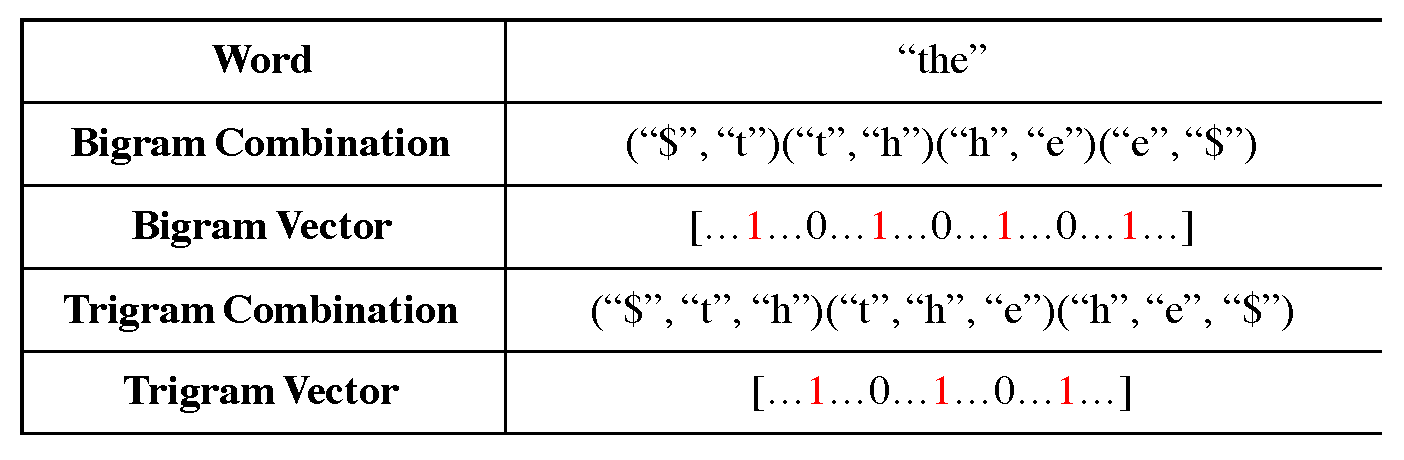
\epsfig{file=pic/bitri.eps, width=0.9\columnwidth}
%	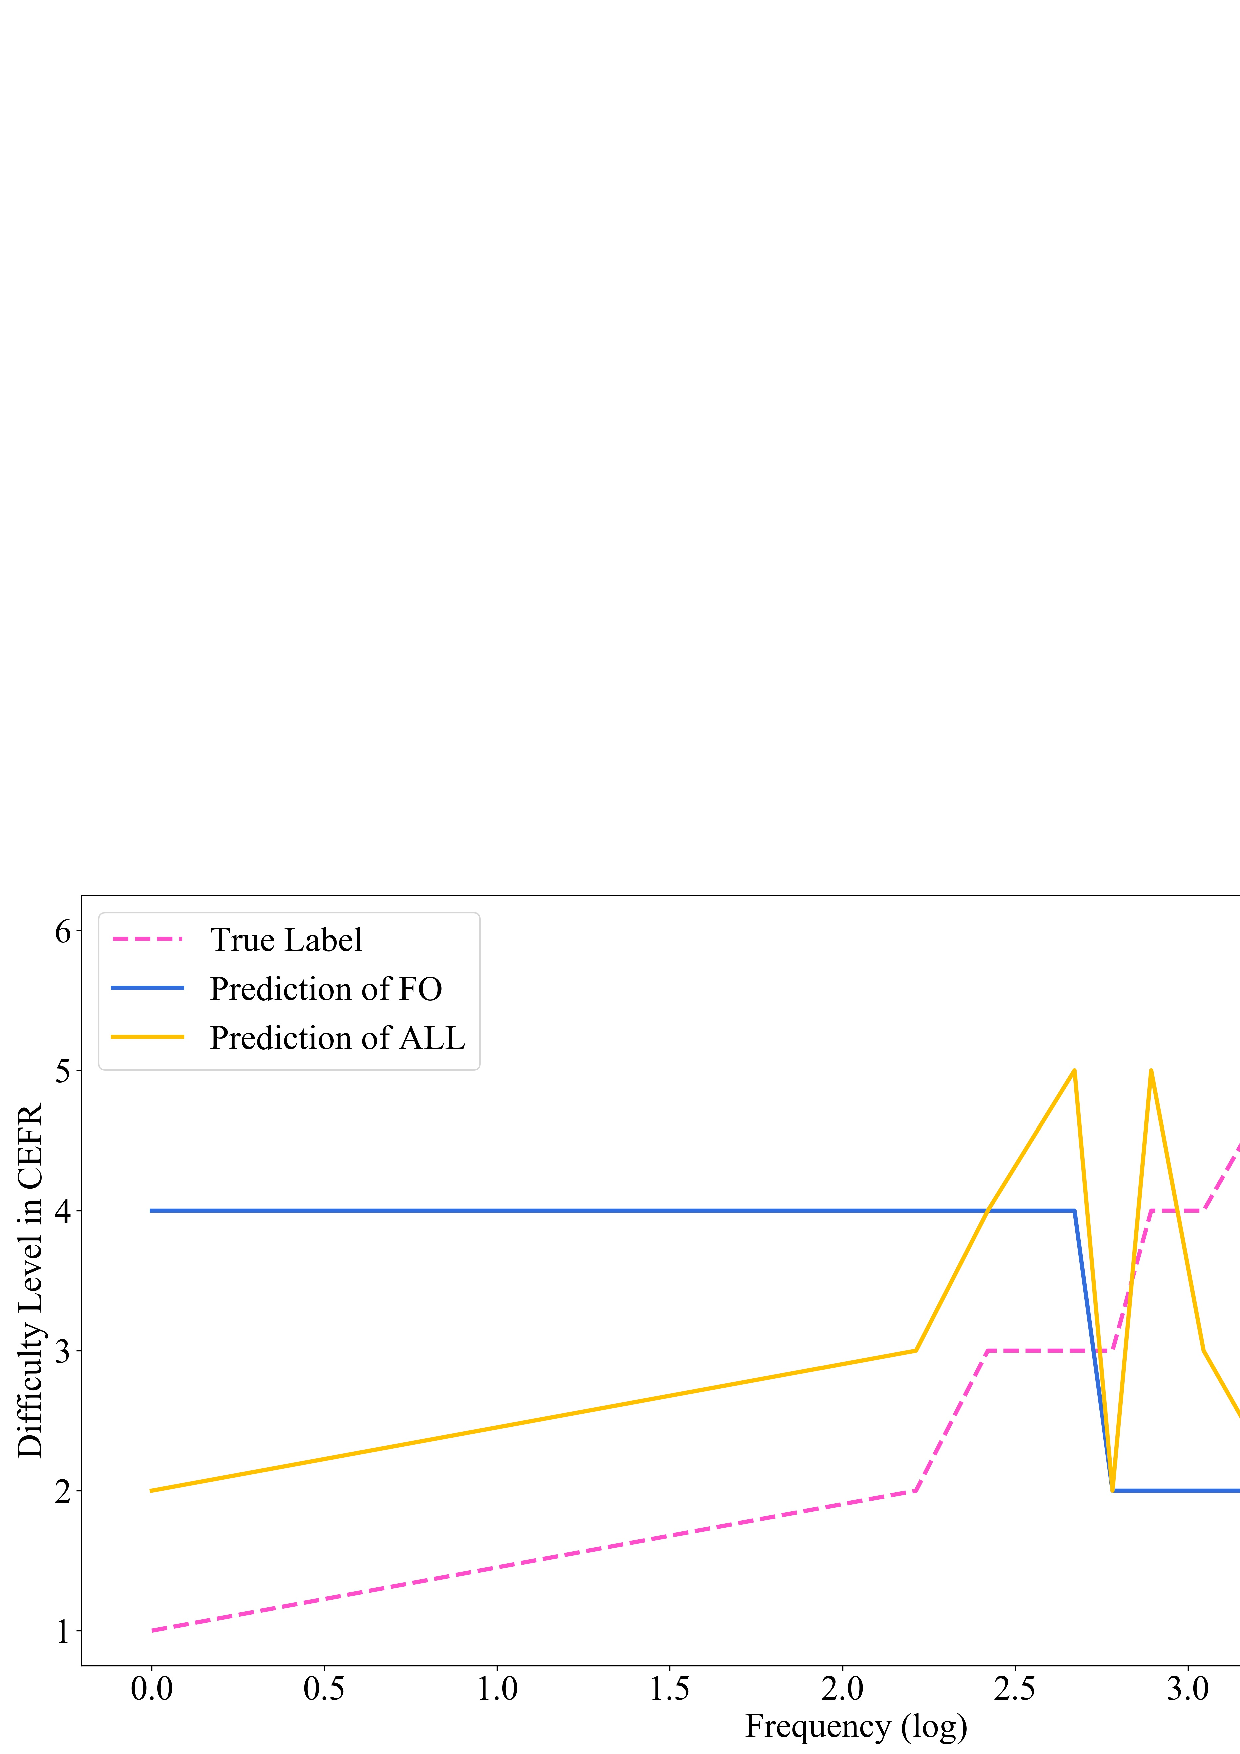
\includegraphics[width=0.5\linewidth]{pic/distance.pdf} 
%	\caption{The relation between log frequency and CEFR levels.
%					Lines show the distance between ground truth and wrongly predictions by FO and Fix+Word2Vec.}
%	\label{fig:distance}
%\end{figure}
%The above results show the prediction of our multi-faceted model (Fix+Word2Vec) is more closer to the ground truth.
%The correlation coefficients in Table \ref{tab:coefficients} also indicates our predictions have a certain correlation with the ground truth compared with baseline model FO.
%\begin{table}[th]
%	\centering
%	\scriptsize
%	\begin{tabular}{|c|c|c|}
%		\hline
%		& \textbf{Pearson} & \textbf{Spearman} \\ \hline
%		\textbf{Ground Truth\&FO} & -0.057 & -0.092 \\ \hline
%		\textbf{Ground Truth\&Fix+Word2Vec} & 0.305 & 0.300 \\ \hline
%	\end{tabular}
%	\caption{\label{tab:coefficients} Correlation coefficient table.}
%\end{table}

%The average accuracy of human classification evaluation is 49.28  for English and 44.44  for German.
%As for difficulty ranking task, the average accuracy of human evaluation is 88.89  for English and 65.85  for German.
%%For English, the accuracy of human labeling is 49.28  and for German, there is an accuracy of 44.44 .
%%That is to say, human can get the correct difficulty level of words with a chance of over 45 . As a result, our work is meaningful because it proves that people can't get a high accuracy by understanding the difficulty level of words in a short time.
%That is to say, it is a truly difficult task that even human can not achieve high accuracy given limited training. 
%In this way, our model 
%which achieves an accuracy around 45 on classification task and 75 on ranking task for both languages is considered very strong.
%Specifically, in English, the accuracy on classification and ranking tasks is close to human behavior.
%In German, the performance of our multi-faceted features is better than human.
%%This result indicates that figuring out the difficulty levels manually with a short-time training is a truly difficult task. 
%%In English, the classification results of multi-faceted are very close to human accuracy. 
%That is to say, our work is once again shown to be meaningful and there is still room for improvement.
%\SY{+Chinese}

\SY{Comparing both the classification and ranking results with human baseline, it is observed that}

\subsection{Ablation Test and Feature Selection}
% and Robustness in Different Corpora
\label{sec:embedding}
Based on the extracted features, we use the multi-layer perceptron (MLP) to investigate the effectiveness of each single feature and their combination MFF.
%We denote the combination of all the features as ALL.
%Then the performance of each individual feature is measured by removing it from MFF one at a time.

\begin{table}[ht]
	\scriptsize
	\setlength{\abovecaptionskip}{0pt}
	\setlength{\belowcaptionskip}{0pt}
	\begin{center}
		\begin{tabular}{lcccc}
		\toprule[1pt]
		&\textbf{NY Times} & \textbf{Gutenberg} & \textbf{German} & \textbf{Chinese} \\ 
		\midrule
	\textbf{MFF}&     \textbf{42.94 }       &   \textbf{41.18 }   &\textbf{47.74 }     &    \textbf{56.96} \\ 
	\midrule
		\textbf{MFF-Freq}     &      40.81     &     40.51 &      47.12      &  51.64  \\ 
	\textbf{MFF-Length}      &    41.72  &  40.90       &  43.00       &  52.36 \\ 
	\textbf{MFF-Phoneme}   &       42.32         &   40.14     &      41.98       &   54.96    \\ 
	\textbf{MFF-BiVec}    &        42.85   &40.77 &       43.00     &    56.70   \\ 
		\textbf{MFF-TriVec}   &         41.28  &   41.11   &46.71     &    55.92   \\ 
	\textbf{MFF-BiProb}    &          42.04     &       38.98   &      45.06        &   56.10  \\ 
		\textbf{MFF-TriProb}  &    41.46         &	39.61       &       45.88      &  52.42   \\ 
	\textbf{MFF-POS}      &      40.70      &      40.93   &       43.21   & 55.32 \\ 
	\textbf{MFF-Dependency}&     38.65               &  37.52   &      46.71      &   55.20    \\ 
		\textbf{MFF-Embedding} &34.22                  & 33.78      & 41.36     &   45.16  \\ 
		\bottomrule[1pt]
	\end{tabular}
	\end{center}
\caption{\label{tab:featurecompare} Classification ablation test of accuracy with each individual feature taken away. 
	Accuracy shown is the average of ten runs. The embedding in this table is Word2Vec.}
\end{table}

Table \ref{tab:featurecompare} shows the classification results of MFF
% and the different compounds with each individual feature taken away.
and each individual feature which are measured by removing it from MFF one at a time,
%In this table, we use Word2Vec to get the word embeddings.
%\SY{Do we need to mention the other embeddings?}
%, because it has a better performance than the other two embeddings which will be shown in the Appendix.
then we find MFF has the best performance.
The lower accuracy of a compound with certain individual feature taken away, the more effective this feature is.
%The most effective features are bolded in all columns.
Then it is observed that 
%We have once again confirmed that 
word frequency is not the determining factor for word difficulty.
% and this phenomenon is more pronounced in German.
%Under both English corpora, the embedding and dependency are top-two effective features.
%While in German, although embedding is still the best feature, we find that the intra-word features of words have a competitive performance.
%\SY{Chinese}
For English, German and Chinese, word embedding is most effective for word difficulty,
while other features behave differently in different languages.
%To show the correctness of the above discovery, 
To investigate the effectiveness of  features under different languages, 
we intuitively conduct the experiments on combination of features in different aspects, 
and the results are in Table \ref{tab:featureL}.

\begin{table}[ht]
	\scriptsize
	\setlength{\abovecaptionskip}{0pt}
	\setlength{\belowcaptionskip}{0pt}
	\begin{center}
		\begin{tabular}{lcccc}
		\toprule[1pt]
		\textbf{}            & \textbf{NY Times}& \textbf{Gutenberg} & \textbf{German} & \textbf{Chinese} \\
		\midrule
		\textbf{MFF}       &      \textbf{42.94}       &   \textbf{41.18}   &\textbf{47.74}    & \textbf{56.96}  \\
		\midrule
		\textbf{Frequency+Length} &      34.13        &      29.55        &      36.05    & \textbf{55.54}  \\ 
		\textbf{Intra-word Features} &      28.14        &      28.45        &      \textbf{44.32}     & 41.82  \\ 
		\textbf{Syntactic Features}     &      31.51        &      30.56        &      39.34    &   52.28  \\ 
		\textbf{Semantic Feature}       &      \textbf{39.40}       &      \textbf{36.82}       &      37.82     & 52.40   \\ 
		\bottomrule[1pt]
	\end{tabular}
	\end{center}
\caption{\label{tab:featureL} Comparison of classification accuracy on different feature aspects on three languages.
Each accuracy is the average of ten runs. The embedding in this table is Word2Vec.}
\end{table}
 
This experiment makes an discovery that intra-word features play a very important role in German words, 
%even though in English it doesn't seem to be as important as other features. 
then frequency and length plays an important role in Chinese words.
%One reasonable explanation is that the pronunciation of German words is closely related to its difficulty which can be 
%discovered in Table \ref{tab:featurecompare} and German words are usually 
%longer than English ones. \SY{+Chinese}
One reasonable explanation is that the pronunciation of German words is closely related to its difficulty which can be 
discovered in Table \ref{tab:featurecompare}.
For Chinese, the construction of HSK vocabulary fully considers the role of frequency.
In addition, it shows that the length of words increases with difficulty level, following the statistical mapping 
\{H1: 1.50, H2: 1.64, H3: 1.78, H4: 1.86, H5: 1.89, H6: 2.04\}.
For English, 
comparing the features extracted from NY Times and Gutenberg, the relative strength of different feature aspects are similar, suggesting strong robustness of the model against different environments.

%According to the results in Table \ref{tab:featurecompare}, word embedding extracted by Word2Vec is the strongest feature to identify word difficulty, so we will consider the effectiveness of  other word embedding models in later contrast experiments on classification and word-pair ranking tasks.

The results in Table \ref{tab:featurecompare} and \ref{tab:featureL} shows the obvious advantages of word embeddings, 
then we design experiments to investigate the performance of different embeddings.
Table \ref{tab:embedding} is the classification result for MFF with different embeddings, such as Word2Vec, GloVe and BERT.
The best results appear between Word2Vec and BERT, but there is no obvious advantages on BERT.
%trend on BERT.
When analyzing the features of different embeddings, we will find that Word2Vec and GloVe combine all the different senses of word into one fixed vector. 
Different from the traditional word embedding algorithms, BERT model can capture the context of a word and clearly distinguish polysemy of a word in the sentence-level tasks.
However, when applying it to word level,  each word is represented with a fixed vector which mixes all the contextual information together and the advantage of BERT model has been defeated.
\begin{table}[ht]
	\scriptsize
	\setlength{\abovecaptionskip}{0pt}
		\setlength{\belowcaptionskip}{0pt}
	\begin{center}
		\begin{tabular}{lcccc}
		\toprule[1pt]
		\textbf{}            & \textbf{NY Times}& \textbf{Gutenberg} & \textbf{German} & \textbf{Chinese} \\
		\midrule
		\textbf{MFF[Word2Vec]} &   \textbf{42.94 } & 41.18  & \textbf{47.74 } &   \textbf{56.96}    \\ 
		\textbf{MFF[GloVe]} &    36.80  & 38.77  & 46.91  &   56.22   \\ 
		\textbf{MFF[BERT]}     &   42.11  & \textbf{41.76 } & 46.30  &  53.78   \\ 
		\bottomrule[1pt]
	\end{tabular}
	\end{center}
\caption{\label{tab:embedding} Classification results with the features including different embeddings.}
\end{table}



\section{Analysis}

We present preliminary statistical findings from ShibaScript, including lexical analysis and transcribing accuracy evaluation.
% \KZ{rewrite this preamble, it's irrelevant now: To give a detailed picture about our dataset ShibaScript and also show several statistical syntax results on it, we will explain our analysis below.}

% This is the analysis on this dataset. Inlcuding its distribution and some further analysis inlcuding bigrams.

% \subsection{Source Information}
% \label{sec:sourceinformation}
% The 16 dogs come from 16 different Japanese user accounts at YouTube. From the videos uploaded from the specific user and the captions attached to these videos, we can get to know much about the growing up environments of dogs, which will influence the expressions of these dogs to some degree. %The environments of them are in \ref{tab:sourceinformation}.
%这是狗的来源的信息,包含地区、是否家养、之类的

% \begin{table}[th]
% \centering
% \begin{tabular}{c|c|c|c}
% \hline
% \textbf{Dog Index} & \textbf{Color} & \textbf{Other Pets} & \textbf{Area}\\\hline
% 0 & yellow & \\
% 1 & yellow & \\
% 2 & yellow & \\
% 3 & yellow & \\
% 4 & yellow & \\
% 5 & yellow & \\
% 6 & yellow & \\
% 7 & yellow & \\
% 8 & yellow & \\
% 9 & yellow & True \\
% 10 & yellow & \\
% 11 & yellow & \\
% 12 & yellow & \\
% 13 & yellow & \\
% 14 & yellow & \\
% 15 & black & \\\hline
% \end{tabular}
% \caption{The source information of dogs in ShibaScript. Color means the fur color of the dog. Other Pets means whether the dog is kept with a family with other animals. Area means the living locations of the family.}
% \label{tab:sourceinformation}
% \end{table}



% \begin{table}
% \centering
% \begin{tabular}{c|c|c|c|c}
% \hline
% \multirow{2}{*}{\textbf{DogID}} & \multicolumn{2}{c|}{\textbf{Sentence}} & \multicolumn{2}{c}{\textbf{Word}}  \\
% \cline{2-5}
% {} & \textbf{Num} & \textbf{Length(s)} & \textbf{Num} & \textbf{Length(s)} \\
% \cline{1-5}
% 0 & 346 & 1107.67 & 577 & 363.36\\
% 1 &  158 & 514.24 & 241 & 129.00\\
% 2 & 553 & 1643.00 & 847 & 469.20\\
% 3 &  55 & 171.69 & 123 & 65.52\\
% 4 & 56 & 224.00 & 107 & 94.08\\
% 5 &  115 & 374.58 & 217 & 98.52\\
% 6 & 52 & 157.00 & 77 & 47.72\\
% 7 & 40 & 135.00 & 65 & 27.44\\
% 8 &  135 & 566.03 & 316 & 143.68\\
% 9 & 255 & 795.00 & 408 & 157.08\\
% 10 & 1188 & 4306.00 & 2029 & 1372.52\\
% 11& 188 & 570.94 & 320 & 203.20\\
% 12  & 130 & 562.28 & 257 & 147.00\\
% 13  & 993 & 2930.19 & 1719 & 749.72\\
% 14  & 118 & 350.11 & 324 & 144.76\\
% 15  & 87 & 299.88 & 134 & 101.24 \\\hline
% sum & \textbf{4469} & \textbf{14707.61} & 7761 & 4314.04\\\hline
% \end{tabular}
% \caption{The basic statistical information of ShibaScript.}
% \label{tab:datasetinformation}
% \end{table}




\subsection{Lexical Analysis}
During the transcribing, there are in total 11 types of tokens, in which 9 types are phonetic symbols~(\tabref{tab:alphabet}), the other two are short pauses between words and long pauses between sentences. 

Similar to humans, the length of these tokens contain ample information. The exact lengths of tokens are kept in ShibaScript for concrete analysis. Because the long pauses are largely determined by the scene at that time, the numerical analysis of it will not be included here. 


\begin{table}[th]
\centering
\small
\begin{tabular}{c|c|c}
\hline
\textbf{Symbol} & \textbf{Mean len (s)} & \textbf{Variance (s)}\\
\hline
\verb|[au]| & 0.35 & 0.022 \\
\verb|[a]| & 0.35 & 0.017 \\
\verb|[^]| & 0.34 & 0.017\\
\verb|[u:]| & 0.45 & 0.054\\
\verb|[u]| & 0.35 & 0.030\\
\verb|[i]| & 0.33 & 0.020\\
\verb|[k]| &  0.24 & 0.009\\
\verb|[(w)au]| & 0.34 & 0.018\\
\verb|[en]| & 0.36 & 0.032\\
\verb|short pause| & 0.57 & 0.335\\
\hline
\end{tabular}
\caption{The mean and variance of the duration of 9 phonetic symbols 
and short pauses between words.}
\label{tab:tokenanalysis}
\end{table}

The mean and variance of each token length can be seen in~\tabref{tab:tokenanalysis}. In which we find that almost every phonetic symbol has a similar length of 0.35s or so. Except for the phonetic symbol \verb|[u:]|, which is a prolonged sound owning an average length of 0.45s. While phonetic symbol \verb|[k]| is a relatively short-lived symbol, only having 0.24s average length.

Considering the monogram~(\figref{fig:monogram}) of ShibaScript, we can find that the most frequent symbol is \verb|[en]|, which reaches to 3478 times in ShibaScript, the following two are \verb|[au]| and \verb|[a]|, which reaches  1981 and 2011 times respectively. One of the reasons why \verb|[en]| exceeds much, which is counterintuitive, is that symbols such as \verb|[a]|, \verb|[au]|, \verb|[(w)au]| are divided up. The least frequent symbol is \verb|[k]|, which only reaches 15 times. This is because dogs seldom produce air-sounds like \verb|[k]|.

At the same time, we can find that these phonetic symbols exist in multiple dogs' sounds, showing that these 9 symbols are universal.

\begin{figure}[th]
\centering
\scalebox{0.32}{\includegraphics{monogram.pdf}}
\caption{The occurrences of each monogram. The blue bars show the occurrences across the whole dataset of each monogram in ShibaScript, the green lines show the numbers of dogs producing the symbols, from 1 to 16.}%\KZ{Remove ``Monogram Stats'' from the pic, since
% you already talk about it in the caption.}
\label{fig:monogram}
\end{figure}

%静音片段分析
%unigram, bigram分析
After analyzing the monogram, we come to find the relationship between symbols, as well as the bigram~(\figref{fig:bigram}) of ShibaScript. Among these bigrams, several appear extremely frequently. It shows a possibility that they are associated with some common semantic meanings. We will dive into that in the future works. Due to space constraints, the detailed information of bigram is shown in~\secref{sec:appendixc}.

% 1 
\begin{figure}[th]
\centering
\scalebox{0.32}{\includegraphics{bigram.pdf}}
\caption{The occurrences of each bigram. The blue bars show the occurrences across the whole dataset of each monogram in ShibaScript, the green lines show the numbers of dogs producing the symbols, from 1 to 16.}
\label{fig:bigram}
\end{figure}




\subsection{Accuracy of Transcription}
In this paper, we discover the certain phonetic pattern of Shiba Inu dogs and assign a vocal dictionary of 9 symbols, which is a first-step trial in this area. To better evaluate the phonetic symbols set as well as the integral accuracy of our transcribing, we have done an evaluation test on these two aspects. The evaluation metric is 5-level Mean Opinion Score~\cite{viswanathan2005measuring}. Three raters will give scores to either one syllable or one word according to~\tabref{tab:ratestandard}. %\MY{How many raters?}


\begin{table}[th]
\centering
\small
\begin{tabular}{c|l}
\hline
\textbf{Score} & \textbf{Description} \\
\hline
5 & The label exactly matches up.\\
4 & Some difference exists between the\\
{}& label and the sound. Humans are s- \\
  & ometimes hard to distinguish.\\
3 & Difference exists between the label\\
  & and the sound. Humans can tell the \\
  & difference immediately.\\
2 & Although the label is obviously wr-\\
{}& ong, there is similarity between t-\\
{}& he label and the sound.\\
1 & The label is totally wrong. \\
% 5 - Excellent 完全一致,失真程度不可察觉
% 4 - Good 有轻微不一致,失真程度略可察觉,如a和ao, u和u:,(w)au 和au,人耳有时也会难以分辨其中差异
% 3 - Fair 一般,失真程度可察觉,人耳可以轻松分辨出二者差异
% 2 - Poor 差,失真程度尚可接受,可以找到一丝相似
% 1 - Bad 很差,失真程度难以接受, 完全不同
\hline
\end{tabular}
\caption{The evaluation metric of rating, which is similar to MOS in speech synthesis evaluation metric.}
\label{tab:ratestandard}
\end{table}

\subsubsection{Phonetic Symbol Accuracy Evaluation}
\label{sec:phone_eva}
%在音素层面进行的evaluation
For each syllable category, we select 50 syllables randomly. The rating result is in~\figref{fig:phoneticaccuracy}. The Fleiss Kappa~\cite{kilicc2015kappa} between three annotators is 0.609.

\begin{figure}[th]
\centering
\scalebox{0.30}{\includegraphics{phoneticaccuracy.pdf}}
\caption{The evaluation result of 9 phonetic symbols. }
\label{fig:phoneticaccuracy}
\end{figure}

% \KZ{Fonts too small, and the image is not clear. Every image must be critical clear after ampification. Use vector images (not bitmap) whenever possible.}

\subsubsection{Word Accuracy Evaluation}
%在word层面进行的evaluation
For the word accuracy evaluation, we select 30 words for each dog randomly and find the same person who rates for phonetic symbols to score for them. The rating result is in~\figref{fig:wordaccuracy}. The Fleiss Kappa between three annotators is 0.516.

\begin{figure}[th]
\centering
\scalebox{0.29}{\includegraphics{wordaccuracy.pdf}}
\caption{The evaluation result of words for 16 different dogs.}
\label{fig:wordaccuracy}
\end{figure}


\section{System Guide}
\label{sec:readme}

Here we give a simple introduction about how to use our codes.

\subsection{Paragraph Retrieval}
\subsubsection{BERT Fine-tuning}
BERT is a pre-trained model and we only need to fine tune it for classification.
The data is under the path ``data/data\_with\_aspect''. 
When training a fine-tuned BERT, you should specify the path of the data in ``bert/ranking.sh'' and run ``bash bert/ranking.sh''.
\subsubsection{TF-IDF, BM25 and BERT}
We implemented the retrieval methods of TF-IDF, BM25 and BERT in the folder ``paragraph\_retrieval/Retrieval''.
Run ``python retrieval\_evaluation.py'' and you can get the retrieval results.
\subsection{Answer Extraction}
\subsubsection{NER}
In "prepro.py", "merge\_raw" function will create the training and test files. Since NER model is pretrained, we don't need to train this model. NER model is from spacy. Just run "python main.py --desc [model name] [--n\_epoch [n\_epoch]] --extract" to test model on test set. Detailed setting can be found in "config.py". You can find more details in readme file.
\subsubsection{BiLSTM-CRF}
For data preprocess, it uses BERT tokenizer to do the tokenization.
First, you need to run ``python make\_NER\_data\_with\_hint.py'' to obtain the tokenized data and transform the answer spans into "BIO" labels.
Then, you should run ``python run\_bilstm\_crf.py  --data\_dir [data path]  --output\_dir [model save path] --do\_train  --use\_sent --max\_seq\_length [max sequence length] --train\_batch\_size [batch size for train]'' to train the model and run ``python ner/run\_bilstm\_crf.py \
    --data\_dir [data path] --output\_dir [model save path]     --do\_test     --eval\_all\_checkpoints     --use\_sent'' to evaluate the model.
\subsubsection{Pointer Network}
First, you need to download glove word embedding into the specific directory.
Then, run ``python build\_data.py'' to obtain the preprecessed data files.
You can train the model by running ``python train.py'' and evaluate the model ny running ``python evaluation.py''.

\subsection{Question Generation}
\subsubsection{Seq2Seq}
The source data is stored in "squad\_hint" directory. First you need to run "process\_data.py" in "data" directory. You may need to download some pretrained word embedding in this step. After data process, you need to specific parameters in "config.py". For example "use\_aspect" determined whether to use aspect in the model. Set "train" as "True" to train the model and "False" to test model on test set. You can find more details in readme file.

\subsubsection{UNILM}
UNILM is a pretrained language model. Here we just use it without changing the model structure. The source data is stored in ``src/qg\_data/raw" directory. In ``data\_process.py", ``process\_data\_hint" and ``process\_data\_no\_hint" will generated the training data with/without aspect. ``process\_data\_test\_annoted" and "process\_data\_test\_annoted\_no\_hint" will generated the testing data with/without aspect. The others are the same as the original unilm model's. Except two differences: we train our model with half-precision(which is much faster) and we train our model in 8 epochs(The result is almost the same compare with 10 epochs).You can find more details in readme file.
\subsection{End-to-end}
\subsubsection{Pipeline Method}
You can run ``python evaluation\_for\_annotation.py'' or ``python evaluation\_for\_annotation2.py'' to get the pipeline results.
There are several parameters need to set before running. If ``do\_decode'' is true, you can generate the QA pairs, and if it's set as false, you can obtain the evaluation results.
Different individual modules can be set in parameter list ``retrieval\_model'', ``an\_model'' and ``qg\_model''.

\subsubsection{Filtering Method}
For the filtering model with retrieval module, you can only run ``python filter.py --qa\_path [path of QA generated by pipeline] --filter\_path [path to store the QAs after filtering]'' after pipeline.
For the filtering model without retrieval module, you should first run ``python filter\_baseline.py --qa\_path [path to store the generated QAs]'' to obtain the QA pairs for all paragraphs, then run ``python filter\_and\_eval.py --qa\_path [path to store the generated QAs] --filter\_path [path to store the QAs after filtering]'' to remove the irrelevant QAs and evaluate the results.
You can find more details in readme file.


\section{Related Work}
This section surveys previous works on question generation and tree encoding
respectively.

Text question generation has attracted the attention 
after the work of ~\citeauthor{du2017learning}~\shortcite{du2017learning}, who uses deep seq2seq model 
to generate questions from a raw text paragraph. 
Before that, text question generation relied heavily on hand-craft 
question patterns~\cite{HeilmanS10,LabutovBV15,MostowC09} which is time and 
labor consuming. 

However, this pure seq2seq model is not focused and 
has no control over part in the paragraph to generate question. 
~\citeauthor{zhou2017neural}~\shortcite{zhou2017neural} proposed to encode 
key phrase information using binary indicators to generate 
key-aware questions and they assumes the answer to be key phrase. 
Considering key phrase (answer) is unavailable in reality, 
~\citeauthor{SubramanianWYT17}~\shortcite{SubramanianWYT17} applied 
a two-stage approach. First, key phrases are extracted by 
pointer network~\cite{ptrnet}. Second, 
key phrases are encoded in the same way as 
Zhou et al. With the intuition that questions could be asked in many ways, 
~\citeauthor{Yao2018vae}~\shortcite{Yao2018vae} used conditional-VAE to 
increase the diversity of questions. More recently, models with 
auxiliary feature information~\cite{HarrisonW18} helped improve 
the question quality. Structure question generation aims at 
converting structured data such as triples in knowledge graph to questions. 
~\citeauthor{SerbanGGACCB16}~\shortcite{SerbanGGACCB16} proposed a model to generate factoid questions from knowledge base triples.  None of the above work
considered using parse tree structures to aid question generation process,
which is the focus of this paper.

Sequential RNN model takes sentence as a sequence of words, 
ignoring the syntactic information. In order to utilize
such syntactic information with sequential information, 
~\citeauthor{tai2015improved}~\shortcite{tai2015improved} proposed Tree-LSTM to 
encode the binary parse tree recursively in a bottom-up fashion to 
classify sentiment. In text generation task, 
\citeauthor{eriguchi2016tree}~\shortcite{eriguchi2016tree} 
proposed a tree-to-sequence model with attention mechanism to do 
machine translation and 
~\citeauthor{liang2018automatic}~\shortcite{liang2018automatic} proposed a 
tree-to-sequence model which could handle arbitrary trees, 
to do code comment generation. Our work is inspired by these previous
attempts and we are first to adapt structure encoded neural models to
textual question generations.

\section{Conclusion}
\label{sec:conclude}
In this work,
we propose a new data creation method to generate
 a semi-structured synthetic training data for 
opinion summarization,
which is known for lacking training data.
\cut{We showed that by extracting an aspect-opinion pairs and 
implicit sentences from multiple reviews
first and then synthesizing them into semi-structured data, we achieve
better performance on opinion summarization.}
%\KZ{It is critical to show in your experiments that the proposed
%synthetic data is better than other possible alternatives.}, 
We also designed an aspect-guided model with opinion-aspect pair encoder and implicit sentence encoder.
The results showed that
the proposed model can make full use of semi-structured data
and generate high-quality summaries.





%% The file named.bst is a bibliography style file for BibTeX 0.99c
\bibliographystyle{ijcai20}
\bibliography{ijcai20}

\end{document}

